% options:
% thesis=B bachelor's thesis
% thesis=M master's thesis
% czech thesis in Czech language
% english thesis in English language
% hidelinks remove colour boxes around hyperlinks

\documentclass[thesis=M,english]{FITthesis}[2018/10/20]

% \usepackage[utf8]{inputenc} % LaTeX source encoded as UTF-8
% \usepackage[latin2]{inputenc} % LaTeX source encoded as ISO-8859-2
% \usepackage[cp1250]{inputenc} % LaTeX source encoded as Windows-1250

\usepackage{graphicx} %graphics files inclusion
\usepackage{listings}
% \usepackage{subfig} %subfigures
% \usepackage{amsmath} %advanced maths
% \usepackage{amssymb} %additional math symbols

\setcounter{tocdepth}{3}% Include \substryAubsection in ToC


\usepackage{dirtree} %directory tree visualisation

% % list of acronyms
% \usepackage[acronym,nonumberlist,toc,numberedsection=autolabel]{glossaries}
% \iflanguage{czech}{\renewcommand*{\acronymname}{Seznam pou{\v z}it{\' y}ch zkratek}}{}
% \makeglossaries

% % % % % % % % % % % % % % % % % % % % % % % % % % % % % %
% EDIT THIS
% % % % % % % % % % % % % % % % % % % % % % % % % % % % % %

\department{Department of System Programming}
\title{GNU-R Debugger Bytecode Support}
\authorGN{Ale{\v s}} %author's given name/names
\authorFN{Saska} %author's surname
\author{Ale{\v s} Saska} %author's name without academic degrees
\authorWithDegrees{Bc. Ale{\v s} Saska} %author's name with academic degrees
\supervisor{Ing. Petr M{\' a}j}
\acknowledgements{Thanks to my adviser Petr M{\' a}j for help with reviewing thesis, my code adviser Tom{\' a}{\v s} Kalibera for useful help with the VM code structure, my father for assistance with the submitting of this work, and big thanks to my girlfriend for psychological support and all the tea.}
\abstractEN{This thesis is about analysis and implementation of current bytecode disassembler tool. The second part is describing the current debugger implementation and there is implementation of it's support for bytecode.}
\abstractCS{V n{\v e}kolika v{\v e}t{\' a}ch shr{\v n}te obsah a p{\v r}{\' i}nos t{\' e}to pr{\' a}ce v {\v c}esk{\' e}m jazyce.}
\placeForDeclarationOfAuthenticity{Prague}
\keywordsCS{Replace with comma-separated list of keywords in Czech.}
\keywordsEN{computer language,R,GNU R,bytecode,disassembler,debugger}
\declarationOfAuthenticityOption{1} %select as appropriate, according to the desired license (integer 1-6)
% \website{http://site.example/thesis} %optional thesis URL


\begin{document}

% \newacronym{CVUT}{{\v C}VUT}{{\v C}esk{\' e} vysok{\' e} u{\v c}en{\' i} technick{\' e} v Praze}
% \newacronym{FIT}{FIT}{Fakulta informa{\v c}n{\' i}ch technologi{\' i}}

\setsecnumdepth{part}
\chapter{Introduction}

\section{Motivation and objectives}

Almost everyone who has been trying to write computer program has made some logical mistakes in them. To help to solve them we usually run program step-by-step with debugging tools with some sort of debugger. The \textbf{GNU R} is one of the most widespread used scientific languages across the whole world.

\textbf{GNU R} language is dynamically typed interpreted language which usually means that it needs \textbf{VM} to interpret. There are more ways to internally represent and implement its evaluation. The first one \textbf{Abstract Syntax Tree}~(see~\ref{AST}) evaluation is the most simplest one. To make speedup of its internal evaluation there has been introduced the \textbf{Bytecode}~(see~\ref{BC}) compiler and interpreter in 1998.

\textbf{Abstract syntax tree} which is usually the slowest one has all debugging features already implemented, but since now there was now no way how to analyze and eventually debug the bytecode one. There has been just very basic bytecode disassembler which was showing the data in human unfriendly way with actual no support for real debugging evaluation of bytecode. Also while debugging function instead of supporting debugging inside bytecode mode there is just fallback that switch to \textbf{AST} in case the function is debugged. This is causing potential issues because the code used for debugging can be slightly different than the code used while not-debugging even if it produces the same result. Eventually this can also cause issue when there is an error inside core AST or BC interpreter, and because the debug and non-debug mode is internally using the different code it can cause to confusing and very hard to solve issue.

This work is solving this issue by analyzing problem, suggesting solutions, and implementing them. The solutions include the implementation of more advanced and user-friendly bytecode disassembler tool and implementing of support for the bytecode debugger. This would enable and significantly improve the support for analysis and debugging any program.

At the beginning of the thesis there is introduction into problems of evaluation of dynamic languages followed by the analysis of possible solutions how to implement the bytecode disassembler and the debugger. In the middle of work there is design of current implementation. After tgat there is described what type of testing has been done on the work. At the end there is proposed work for the future improvements of the work followed by thesis summarization in conclusion.

\section{Problem statements}

There are two main types of programming languages. Dynamic typed and static typed ones.
Static such as \textbf{C} / \textbf{C++} / \textbf{FORTRAN} languages has strictly defined types and are usually more machine inspired/focused. Dynamic ones usually do not have strict type inference so they allow the user~(programmer) more freedom. As trade-off they usually needs Virtual Machine~(\textbf{VM}, see~\ref{VM}) to runs efficiently which cause possible performance slowdown. \textbf{GNU R} language was primarily developed for the scientists so user-friendliness and no need to necessary care about data types was one of the decision to make the language dynamic typed.

TODO: add more of some good shit

\setsecnumdepth{all}
%\chapter{State-of-the-art}

\chapter{Analysis and design}

\section{GNU R from user perspective}\label{R-UI}

\subsection{Basis usage~(main commands and REPL loop)}\label{R-UI}

The main \textbf{GNU R} language is written as the console application evaluating the infinite \textbf{REPL} loop. As the abbreviation says, it is evaluating the expressions right as is entered by user~(the \textbf{R} program). Alongside of this there is also the \textbf{Rscript} command in the package which supports running the program from the input file, but it is internally implemented just as wrapper piping the file content into the \textbf{R} command.

\subsection{GNU R package system}\label{R-Packages}

The \textbf{GNU R} has its own integrated package subsystem \textbf{CRAN} with plenty of inbuilt packages. These packages are intended to be easy way for developers~(\textbf{R} users) how to make user friendly extension for other people.

Therese are few basic commands to work with packages:

\begin{itemize}
	\item R CMD INSTALL $<$pkgs$>$ - install specified packages
	\item R CMD build $<$pkgname$>$ - build package
	\item R CMD check $<$pkgname$>$ - check package~(check requirements, run tests etc.)
\end{itemize}



\subsection{GNU R class system}\label{R-Classes}

\textbf{GNU R} Citing the Hadley Wickham's article OO field guide~\cite{R-OO}:

R has s three OO systems differ in how classes and methods are defined:

\begin{itemize}
\item \textbf{S3} implements a style of OO programming called generic-function OO. This is different from most programming languages, like Java, C++, and C{\#}, which implement message-passing OO. With message-passing, messages~(methods) are sent to objects and the object determines which function to call. Typically, this object has a special appearance in the method call, usually appearing before the name of the method/message: e.g., \textit{canvas.drawRect("blue")}. S3 is different. While computations are still carried out via methods, a special type of function called a generic function decides which method to call, e.g., \textit{drawRect(canvas, "blue")}. S3 is a very casual system. It has no formal definition of classes.

\item \textbf{S4} works similarly to S3, but is more formal. There are two major differences to S3. S4 has formal class definitions, which describe the representation and inheritance for each class, and has special helper functions for defining generics and methods. S4 also has multiple dispatch, which means that generic functions can pick methods based on the class of any number of arguments, not just one.

\item \textbf{Reference classes}, called RC for short, are quite different from S3 and S4. RC implements message-passing OO, so methods belong to classes, not functions. {\$} is used to separate objects and methods, so method calls look like \textit{canvas{\$}drawRect("blue")}. RC objects are also mutable: they don't use R's usual copy-on-modify semantics, but are modified in place. This makes them harder to reason about, but allows them to solve problems that are difficult to solve with S3 or S4.


There's also one other system that's not quite OO, but it's important to mention here:


\item \textbf{base types}, the internal C-level types that underlie the other OO systems. Base types are mostly manipulated using C code, but they're important to know about because they provide the building blocks for the other OO systems.
\end{itemize}

Basically it means that the \textbf{R} class system is not strictly defined as in languages like \textbf{Java}, \textbf{C++}, \textbf{Python} etc. The whole system provides the end user to more flexibility, but on the other hand it can be little bit more confusing for the programmers which are used to regular programming languages.

\section{GNU R internal structure}\label{R-internal-structure}

The core \textbf{GNU R} VM core is written in C language with the broad number of supported platforms~(Windows/MAC/Linux...) and computer architectures~(ARM/x86/x64...).

\subsection{Implementation of the core features of language in R itself}

The \textbf{GNU R} has internally written the loading mechanism in the way that the \textit{"base"} package is loaded first and then all of the packages contained in list \textit{getOption("defaultPackages")} are loaded into the global environment. These mechanism allows that just the core features and language constructs are written in performance optimized \textbf{C} and the rest can be written inside \textbf{R} language itself. It means that inside these packages there is a lot of functionality for the whole language environment.

\subsection{Calling internal C functions from R}

\textbf{C} code compiled into \textbf{R} at build time can be called directly in what are termed primitives or via the \textbf{.Internal} interface, which is very similar to the \textbf{.External} interface except in syntax. More precisely, \textbf{R} keeps a table of function names and corresponding C functions to call, which by convention all start with \textit{do{\_}} and return a \textit{SEXP}. This table (\textit{R{\_}FunTab} sitting in file \textit{src/main/names.c}) also specifies how many arguments to a function are required or allowed, whether or not the arguments are to be evaluated before calling, and whether the function is \textit{internal} in the sense that it must be accessed via the \textbf{.Internal} interface, or directly accessible in which case it is printed in \textbf{R} as \textbf{.Primitive}.

\section{Computer Program Compiler Structure}

\subsection{Internal structure}\label{Compiler-internal-structure}

To make compilers structure internally more organized most of the compilers or \textbf{VM}s are divided into separate passes.

The common basic ones are:
\begin{itemize}
	\item Frontend - parsing source code into \textbf{IR} or \textbf{AST}~(see chapter~\ref{AST} )
	\item Optimizer - optimizing \textbf{IR} or \textbf{AST}~(can be left out)
	\item Backend - generating machine code or running \textbf{VM}~(see chapter~\ref{VM})
\end{itemize}
Each step can be also divided into more steps (for example frontend consists usually of lexer and parser).

As long as the \textbf{GNU R} is dynamic language it is build over the internal Virtual Machine. It does an on-demand parsing of the source code which directly evaluates.

The optimization problem is very difficult inside the \textbf{GNU R}. One of its' example why this is not possible is extreme dynamism of the language. For example you can:
\begin{itemize}
	\item Change the body, arguments, and environment of functions.
	\item Change the S4 methods for a generic.
	\item Add new fields to an S3 object, or even change its class.
	\item Modify objects outside of the local environment with <<-.
\end{itemize}

Basically the \textbf{GNU R} is monolithic structure built in over the Virtual Machine. This design is not ideal but it came up from to historic reasons.

\subsection{Virtual Machine}\label{VM}

As long as the \textbf{GNU R} is the dynamically typed computer language it needs the \textbf{Virtual Machine} to runs on. Static compiled languages use as the environment directly the computer operating system.
On the other hand the \textbf{Virtual Machine} is simulating the environment by executing code, managing memory, and providing communication layer with the underlying computer and it's external devices ( accessing filesystem, network communication etc. ). This means there is performance slowdown but on the other hand there is big safety advantage of isolation which means that you cannot write the harmful code that interacts directly with the underlying system.

There are more types of virtual machines. The most common ones are stack machines followed by the register based machines.

The \textbf{register based} ones simulates register processors (such as \textbf{x86} architecture Intel or \textbf{ARM} ones) with instructions having more registers to get internally values from. This implicates more sophisticated instruction coding because each one has to also have encoded what registers should be used as input for the instruction ( for example Android \textbf{Dalvik VM} add-int instruction has 3 parameters - Destination parameter, first source register, and second source register ). This results in longer instruction sizes and more expensive instruction decoding which both negatively impacts execution speed.

The \textbf{stack based} ones on the other hand are simpler ones because every instruction arguments lies on the top of the stack in the specified order (for example ADD instruction removes two topmost arguments from the top, make addition, and push result back to the top of the stack). This implies much easier instructions and also easier implementation of whole compiler and evaluator.

The examples of virtual machines are
\begin{itemize}
	\item JVM - Java VM
	\item Python
	\item GNU R
	\item Dalvik VM - Android VM ( the only register one based in this list )
	\item JavaScript V8
	\item Chakra ( JavaScript inside MS Edge browser)
\end{itemize}



\textbf{GNU R} virtual machine is register based one with one byte size bytecode instructions. Due to simplicity it consists of these parts:
\begin{itemize}
	\item \textbf{Parser} (mainly in src/main/gram.y which generates src/main/gram.c)
	\item \textbf{Memory management} ( mainly in src/main/memory.c )
	\item \textbf{AST evaluator} ( eval function inside src/main/eval.c )
	\item \textbf{Bytecode Compiler} ( inside R package Compiler )
	\item \textbf{Bytecode evaluator} ( bcEval function inside src/main/eval.c )
	\item etc.
\end{itemize}

\subsection{Garbage Collector}\label{GC}

Memory management in dynamic languages is maintained by  \textbf{Garbage Collector}. It releases allocated memory once it is no longer used. \textbf{GNU R} implementation of memory management lies inside src/main/memory.c. It implements a non-moving generational garbage collector with two or three generations. Memory allocated by \textit{R{\_}alloc} is maintained in a stack. Code that \textit{R{\_}alloc}ates memory must use \textit{vmaxget} and \textit{vmaxset} to obtain and reset the stack pointer.

Each memory node is represented as \textit{SEXP} type. It contains internal representations such as code definition ( \textit{LANGSXP}, \textit{BCOSESXP}, \textit{WEAKREFSXP}, promises etc. ) and also regular memory types (such as logical vectors, integer vectors, strings vectors etc.). \textbf{GNU R} is internally an vector language so every value is internally represented as vector (e.g. integer 3 is represented and boxed as \textbf{INTSXP} vector of size 1 containing value 3).

Types of memory nodes are

\begin{itemize}
	\item \textbf{NILSXP} nil = NULL
	\item \textbf{SYMSXP}	     symbols
	\item \textbf{LISTSXP}	     lists of dotted pairs
	\item \textbf{CLOSXP}	     closures
	\item \textbf{ENVSXP}	     environments
	\item \textbf{PROMSXP}	     promises: [un]evaluated closure arguments
	\item \textbf{LANGSXP}	     language constructs (special lists)
	\item \textbf{SPECIALSXP}   	special forms
	\item \textbf{BUILTINSXP}   	builtin non-special forms
	\item \textbf{CHARSXP}	     "scalar" string type (internal only)
	\item \textbf{LGLSXP}	    logical vectors
% 11 and 12 were factors and ordered factors in the 1990s
	\item \textbf{INTSXP}	    integer vectors
	\item \textbf{REALSXP}	    real variables
	\item \textbf{CPLXSXP}	    complex variables
	\item \textbf{STRSXP}	    string vectors
	\item \textbf{DOTSXP}	    dot-dot-dot object
	\item \textbf{ANYSXP}	    make "any" args work.
%			     Used in specifying types for symbol			     
%			     registration to mean anything is okay
	\item \textbf{VECSXP}	    generic vectors
	\item \textbf{EXPRSXP}	    expressions vectors
	\item \textbf{BCODESXP}    byte code
	\item \textbf{EXTPTRSXP}   external pointer
	\item \textbf{WEAKREFSXP}  weak reference
	\item \textbf{RAWSXP}      raw bytes
	\item \textbf{S4SXP}       S4, non-vector
% used for detecting PROTECT issues in memory.c
	\item \textbf{NEWSXP}      fresh node created in new page
	\item \textbf{FREESXP}     node released by GC

	\item \textbf{FUNSXP}      Closure or Builtin or Special
\end{itemize}

\subsection{Computed GOTO}\label{Computed-GOTO}

The internal representation of \textbf{BC} evaluator inside \textbf{VM} acts like big loop going through all \textbf{BC} instructions of function. In the each loop step there has to be branching of flow according to instruction. In the traditional way this is done as the switch-case where case values are the instruction codes. Example of this approach:

\begin{lstlisting}
while(1){
  switch(*opcode++){
    case POP:	//POP=1
      ... do instruction POP ....
      break;
    case GETVAR:	//GETVAR=2
      ... do instruction GETVAR ....
      break;
    case ADD:	//GETVAR=3
      ... do instruction ADD ....
      break;
  }
}
\end{lstlisting}

The \textit{switch} statement should be implemented very efficiently by \textbf{C} compilers - the condition serves as an offset into a lookup table that says where to jump next. However, it turns out that there's a popular \textbf{GCC} extension that allows the compiler to generate even faster code. The main idea behind this is to store the address of the label into value of variable which allows the dynamic lookup of the next value.

Example of computed-goto code:
\begin{lstlisting}
/* The indices of labels in the dispatch_table 
 * are the relevant opcodes
 */
static void* dispatch_table[] = {
        &&do_halt, &&do_inc, &&do_dec, &&do_mul2,
        &&do_div2, &&do_add7, &&do_neg};
#define DISPATCH() goto *dispatch_table[code[pc++]]

int pc = 0;
int val = initval;

DISPATCH();
while (1) {
    do_halt:
        return val;
    do_inc:
        val++;
        DISPATCH();
    do_dec:
        val--;
        DISPATCH();
    do_mul2:
        val *= 2;
        DISPATCH();
}
\end{lstlisting}

\textbf{GNU R} has the support of threaded code~(implemented by the \textbf{computed GOTO} technique) although there is still support for non-GCC compilers~(and compilers which does not support this feature). Enabing of this feature is managed by (\textit{THREADED{\_}CODE} define macro flag. 

The all of the while loop and switch cases are in the \textbf{GNU R} code then defined with macros~(e.g. \textit{OP}, \textit{BEGIN{\_}MACHINE} etc.). These macros code are conditionally defines to either be compiled to enable or disable support for threaded code. Basically according to the \textit{THREADED{\_}CODE} flag there is conditional two implementations of these macros which enables or disables this functionality.

In the \textbf{GNU R} implementation of bytecode interpreter there is performance optimization associated with dispatch table and the \textbf{computed GOTO}. In process of loading bytecode into the \textbf{VM} internal structure~(done by \textit{R{\_}bcDecode} and \textit{R{\_}bcEncode} inside \textit{src/main/eval.c}) there is translation between instruction codes~(1 byte/char codes) and current location of jump labels inside \textit{bcEval} - see \textit{computed goto}~\ref{AST}(\textit{void*} type). The nature of the operating system loader would cause that this position can~(and usually is) changed every time the program is started~(R is loaded into memory by operating system) - so value has to be computed every time again. This allows \textbf{BC} interpreter to jump directly at the position which is stored inside the \textbf{BC} definition which means saving one array lookup every step of \textbf{BC} interpreter~(\textbf{BC} instruction) compared to the classic interpreter~(implemented for example inside \textbf{cpython} VM).

\subsection{Abstract Syntax Tree}\label{AST}

To be able to internally interpret the syntax of every language the code is first parsed into abstract syntax tree~(\textbf{AST}, example in fig.~\ref{fig:ast-while}). Tree in the \textbf{GNU R} contains nodes of \textit{LANGSXP} type with references to the symbol table~(pointers to the function) which contains function to evaluate the code. This tree is then traversed and evaluated inside eval function which lies in file \textit{src/main/eval.c}. The evaluator also has built-in support for debugging which is done internally by the checking of the \textit{RDEBUG} flag of current executed environment in its every step~(creates performance overhead even though the debug mode is not active).

\begin{figure}\centering
	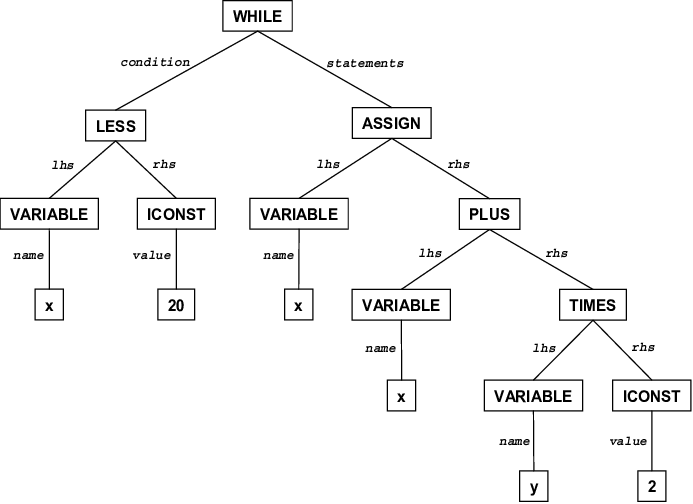
\includegraphics{Abstract-syntax-tree-of-the-while-loop}
	\caption{While loop example}\label{fig:ast-while}
\end{figure}

\subsection{Bytecode}\label{BC}

Another option how to represent the source code to evaluate is the \textbf{bytecode}. It is array of transferable instruction codes and constants designed for easy evaluation. The name bytecode stems from instruction set that have one byte operation code. Structure contains the instruction code which follows parameters ( depending on how many / if parameter given instruction have ).

\subsection{Just in Time compilation}\label{JIT}

In order to speedup evaluation of inside \textbf{VM} there has been developed various techniques of the performance optimization. One of them is Just in Time compilation of code. The underlying idea is to internally translate code into some more efficient representation ( from \textbf{AST} to either \textbf{Bytecode} or to the native machine code ). However this transformation (compilation) is usually pretty expensive so it is called once the execution of specified piece of code reached some limit.
\textbf{GNU R} has basic internal support of \textbf{JIT}. Implementation lies inside src/main/eval.c mainly in functions \textit{R{\_}CheckJIT} and \textit{R{\_}cmpfun} ) and doing running of the \textit{Compiler::tryCmpfun} to compile function \textbf{AST} into \textbf{bytecode}. According to the posts from running code with ByteCode JIT enables speedup up to 10 times~(theoretically up to 25 times but these cases are very rare).

As mentioned before, the compilation can take significant amount time, so it makes sense for the virtual machine to compile just the most used parts of code~(if the every function would be compiled, it would have even cause the slowdown). The \textbf{GNU R} has for this more strategies:

\begin{itemize}
  \item \textit{NO{\_}CACHE}

      functions are compiled 1st time seen

      \hspace*{6mm} code is never cached

  \item \textit{NO{\_}SCORE}

      functions are compiled 1st time seen,

      \hspace*{6mm} code is cached,

      in case of conflict function may be marked \textit{NOJIT}

  \item \textit{ALL{\_}SMALL{\_}MAYBE}

      functions with small score are compiled 2nd time seen,

      function with high score are compiled,

      \hspace*{6mm} 1st time seen if top-level, 2nd time seen otherwise

  \item \textit{TOP{\_}SMALL{\_}MAYBE}

      functions with small score compiled,

      \hspace*{6mm} 2nd time seen if top-level, never otherwise

      functions with high score compiled

      \hspace*{6mm} time seen if top-level, 2nd time seen otherwise
\end{itemize}


\section{GNU R Bytecode}

\textbf{GNU R} has internal support of the \textbf{BC} which consists of Compiler package for compiling to the bytecode and interpreting function \textit{bcEval}~(inside \textit{src/main/eval.c}) which evaluates the \textbf{BC}. Compiler can be used explicitly by calling certain functions to carry out compilations or implicitly by enabling compilation to occur automatically at certain points.

\begin{itemize}
  \item Explicit compilation primary functions are \textit{compile}, \textit{cmpfun}, \textit{cmpfile}
  \item Implicit compilation can be used to compile packages as they are installed or for \textbf{JIT} compilation of functions or expressions.

For now the compilation of packages is enabled by calling \textit{compilePKGS} with argument \textbf{TRUE} or by starting R with the environment variable \textit{R{\_}COMPILE{\_}PKGS} set to positive integer value.
\end{itemize}


\subsection{GNU R internal representation of bytecode}\label{R-internal-bc-representation}

Internal representation of bytecode is wrapped inside \textit{SEXP} node of \textit{BCODESXP} type. It's represented as an linked list with these parameters~(arrays of integers)
\begin{itemize}
	\item \textbf{Bytecode code}~(body) array which contains set bytecode instructions following its' parameters

		\hspace*{6mm} internally represented as first element~(\textit{CAR}) of linked list

		\hspace*{6mm} The array contains char~(1~Byte size) representation of version number followed by the bytecode instructions 

	\item \textbf{Constant pool} array

		\hspace*{6mm} internally represented as second element~(\textit{CDR}) of linked list

\end{itemize}

\subsection{Expression and source references}\label{Exprref-and-srcref}

At the end of the constant pool array there can be~(are optional) some additional information about the bytecode. These information are not used for the evaluation, but are provided for specifying the original location of compiled code. They can be of 2 types:

\begin{itemize}
	\item \textbf{Expression reference}

describing the expression representation of bytecode~(for example \textit{b+a+4})

	\item \textbf{Source reference}

describing the location in the source file~(for example \textit{main.R{\#}4})
\end{itemize}

The data structures in the end of the constant array can contain these class types:

\begin{itemize}
	\item \textbf{srcref}

Source reference representing the whole function~(it's beginning)

	\item \textbf{srcrefsIndex}

Array corresponding source references to code for each instruction~(length of the array is length of BC code array - see~\ref{R-internal-bc-representation})

	\item \textbf{expressionsIndex}

Array corresponding expression references~(expressions) to code for each instruction~(length of the array is length of BC code array - see~\ref{R-internal-bc-representation})

\end{itemize}

\section{Current implementation of AST debugger}\label{AST-debugger}

\textbf{AST} evaluator of \textbf{GNU R} is implemented as recursive descent of the \textbf{AST} tree.
The debugger is made on top of the \textbf{AST} interpreter and it uses the \textit{RDEBUG} flag of current evaluated to check if enable the debugging features. For user there are written functions~(user interface) managing this functionality. They are:

\begin{itemize}
	\item debug(fun, text = "", condition = NULL, signature = NULL)
	\item debugonce(fun, text = "", condition = NULL, signature = NULL)
	\item undebug(fun, signature = NULL)
	\item isdebugged(fun, signature = NULL)
	\item debuggingState(on = NULL)
\end{itemize}

To keep the same debug functionality for functions running on top of the bytecode there is fallback for switching back to the \textbf{AST} implementation. It implicates that for users the code behaves in the same way~(both \textbf{BC} and \textbf{AST} representation are producing equivalent output), but can cause an issues in case of the internal problems~(there is error in either \textbf{AST} or \textbf{BC} evaluator). In that case the code while debugging would be using the different code while not and potentially could have been very confusing. There is also no way to debug \textbf{BC} internals (\textbf{BC} stack and showing the current evaluating instruction in the \textbf{BC}) while running.

The \textbf{GNU R} debugger internal implementation of interacting with user is made internally by calling the \textit{browse()} function which is running the environment browser. Its purpose is to wait for user console input and evaluate it. Its internal representation is reusing the function shared with main \textbf{REPL} loop~(mainly functions \textit{Rf{\_}ReplIteration} and \textit{ParseBrowser} inside src/main/main.c) for support user input~(parsing and evaluating).

The \textit{browse()} function also has support for the commands managing the debug mode. They are:
\begin{itemize}
\item c - exit the browser and continue execution at the next statement.
\item cont - synonym for c.
\item f - finish execution of the current loop or function
\item help - print this list of commands
\item n - evaluate the next statement, stepping over function calls. For byte compiled functions  interrupted by browser calls, n is equivalent to c.
\item s - evaluate the next statement, stepping into function calls. Again, byte compiled functions make s equivalent to c.
\item where - print a stack trace of all active function calls.
\item r - invoke a "resume" restart if one is available; interpreted as an R expression otherwise. Typically "resume" restarts are established for continuing from user interrupts.
\item Q - exit the browser and the current evaluation and return to the top-level prompt.

\end{itemize}

\section{Current implementation of Bytecode disassembler}\label{current-bc-disassembler}

There is already implemented the way how to see bytecode representation - the bytecode disassembler function \textit{disassemble} in \textit{compile} package. Even though its current functionality is very minimal and insufficient. It is very basic and just works the way that converts the code instructions and constant buffer to array and dputs it into the console. It means that the user would see~(the function would return) just two arrays with which is definitely not user friendly. The source code consists of 2 short functions \textit{disassemble} and \textit{bcDecode}:

\begin{lstlisting}
disassemble <- function(code) {
    .CodeSym <- as.name(".Code")
    disasm.const<-function(x)
        if (typeof(x)=="list" && length(x) > 0
        		&& identical(x[[1]], .CodeSym))
            disasm(x) else x
    disasm <-function(code) {
        code[[2]]<-bcDecode(code[[2]])
        code[[3]]<-lapply(code[[3]], disasm.const)
        code
    }
    if (typeof(code)=="closure") {
        code <- .Internal(bodyCode(code))
        if (typeof(code) != "bytecode")
            stop("function is not compiled")
    }
    dput(disasm(.Internal(disassemble(code))))
}

bcDecode <- function(code) {
    n <- length(code)
    ncode <- vector("list", n)
    ncode[[1]] <- code[1] # version number
    i <- 2
    while (i <= n) {
        name<-Opcodes.names[code[i]+1]
        argc<-Opcodes.argc[[code[i]+1]]
        ncode[[i]] <- as.name(name)
        i<-i+1
        if (argc > 0)
            for (j in 1:argc) {
                ncode[[i]]<-code[i]
                i<-i+1
            }
    }
    ncode
}
\end{lstlisting}

\section{Analysis of disassembler improvements}\label{analysis-of-disassembler}
The current implementation of bytecode disassembler is unsufficient so it needs to be improved. In the following paragraphs there is detailed analysis of another implementations of diassemblers and possibility of implementation advanced one inside \textbf{GNU R}.

\subsection{Java bytecode disassembler}

The nice example of disassembler is in Java language~(\textit{javap} command of Java package). The java bytecode is although very specific and each file contains the one class. The whole file contains representation of the file just as the bytecode. Although the \textbf{GNU R} implementation is different - there can be mixed up the non-compiled~(\textbf{AST}) and compiled~(\textbf{BC}) code. It means that the bytecode printer is showing just the one function at once.

Example output of the \textit{javap} command is the:

\begin{lstlisting}
#>javap -c -verbose ./HelloWorld.class
Classfile
 /C:/Users/aless/skola/thesis/java_bc/HelloWorld.class
  Last modified Mar 8, 2018; size 426 bytes
  MD5 checksum 2855c0c8a8386e26943e1bce67c9fc96
  Compiled from "HelloWorld.java"
public class HelloWorld
  minor version: 0
  major version: 53
  flags: (0x0021)
  			ACC_PUBLIC, ACC_SUPER
  this_class: #5
  		// HelloWorld
  super_class: #6
  		// java/lang/Object
  interfaces: 0, fields: 0, methods: 2, attributes: 1
Constant pool:
   #1 = Methodref          #6.#15
   		// java/lang/Object."<init>":()V
   #2 = Fieldref           #16.#17
 // java/lang/System.out:Ljava/io/PrintStream;
   #3 = String             #18
   		// Hello, World
   #4 = Methodref          #19.#20
 // java/io/PrintStream.println:(Ljava/lang/String;)V
   #5 = Class              #21
   		// HelloWorld
   #6 = Class              #22
   		// java/lang/Object
   #7 = Utf8               <init>
   #8 = Utf8               ()V
   #9 = Utf8               Code
  #10 = Utf8               LineNumberTable
  #11 = Utf8               main
  #12 = Utf8               ([Ljava/lang/String;)V
  #13 = Utf8               SourceFile
  #14 = Utf8               HelloWorld.java
  #15 = NameAndType        #7:#8
  		// "<init>":()V
  #16 = Class              #23
  		// java/lang/System
  #17 = NameAndType        #24:#25
  		// out:Ljava/io/PrintStream;
  #18 = Utf8               Hello, World
  #19 = Class              #26
  		// java/io/PrintStream
  #20 = NameAndType        #27:#28
  		// println:(Ljava/lang/String;)V
  #21 = Utf8               HelloWorld
  #22 = Utf8               java/lang/Object
  #23 = Utf8               java/lang/System
  #24 = Utf8               out
  #25 = Utf8               Ljava/io/PrintStream;
  #26 = Utf8               java/io/PrintStream
  #27 = Utf8               println
  #28 = Utf8               (Ljava/lang/String;)V
{
  public HelloWorld();
    descriptor: ()V
    flags: (0x0001) ACC_PUBLIC
    Code:
      stack=1, locals=1, args_size=1
         0: aload_0
         1: invokespecial #1
         	// Method java/lang/Object."<init>":()V
         4: return
      LineNumberTable:
        line 1: 0

  public static void main(java.lang.String[]);
    descriptor: ([Ljava/lang/String;)V
    flags: (0x0009) ACC_PUBLIC, ACC_STATIC
    Code:
      stack=2, locals=1, args_size=1
         0: getstatic     #2
   // Field java/lang/System.out:Ljava/io/PrintStream;
         3: ldc           #3
         	// String Hello, World
         5: invokevirtual #4
 // Method java/io/PrintStream.println:(Ljava/lang/String;)V
         8: return
      LineNumberTable:
        line 4: 0
        line 5: 8
}
SourceFile: "HelloWorld.java"

\end{lstlisting}

\subsection{Python bytecode disassembler}

\textbf{Python} has in-built support of disassembler for it's internal \textbf{BC}. It is provided inside package \textit{dis} which is part of python~(no need to manually installing). Source code location is in the \textit{Lib/dis.py}. As you can see the code is showing just one function at once. It is also showing the combined output of constant array at one line~(not printing any separate array for constant array).

The usage example:
\begin{lstlisting}
import dis

def myfunc(alist):
    return len(alist)

dis.dis(myfunc)
# Generating output
#  2           0 LOAD_GLOBAL              0 (len)
#              2 LOAD_FAST                0 (alist)
#              4 CALL_FUNCTION            1
#              6 RETURN_VALUE

\end{lstlisting}

\subsection{Summary}

The difference between the \textbf{Java} \textit{javap} and the \textbf{Python} \textit{dis} command is that \textit{javap} works on the whole file instead of the Python \textit{dis} which is printing just one function. They both dumps the \textbf{BC} in the human-readable form with instructions line-by-line. The \textbf{Python} one is showing the parameters from the constant pool altogether with the instruction. The \textit{javap} tool on the other hand supports more levels of verbosity.

As long as the R can internally combine in memory \textbf{AST} and \textbf{BC} representation of the code, the way how to disassemble code is just for the one specific function. In case there are a lot of information inside \textbf{GNU R} bytecode it would be also nice to have ability to show these information just as parameters through verbosity level. The inline showing values from the constant pool would be also useful because it can result in compact and shorter output with easily enabling the feature for printing just specified are of function.

\section{Analysis of Bytecode debugger implementation}

Currently there is no support for debugging the bytecode evaluation in real time~(just the fallback to the \textbf{AST} one is present) so there is no current implementation of the BC debugger to go through. Instead of it we can inspire ourselves with the current AST implementation which is done in the first part of this section. The following parts are analyzing the implementation of the \textbf{BC} debugger in other VMs~(\textit{Python} VM and \textit{V8} javascript VM).

\subsection{Inspiration with current AST implementation}
The general idea how to run the is taken from the current implementation of the \textbf{AST} debugger. The example of \textbf{AST} implementation of the debug:
\begin{lstlisting}
if (RDEBUG(rho) && !R_GlobalContext->browserfinish) {
  SrcrefPrompt("debug", R_Srcref);
    //Print "debug" followed by
    //  source reference of the current evaluated code
  PrintValue(CAR(args));
  	//print current evaluated expression
  do_browser(call, op, R_NilValue, rho);
  	//run the environment browser
}
\end{lstlisting}
Basically this code check if there is \textit{RDEBUG} flag on the current executed function and if there is it would print information about the current evaluated code~(source reference if available + evaluated expression). Following command is the \textit{do{\_}browser()} which is internally calling the environment browser with support for evaluating expression~(seeing what is value of which variable + evaluating functions) and inbuilt handling of debugger commands~(\textit{next step}, \textit{step into}, \textit{continue} etc.). It also has support for showing backtrace~(\textit{where} command). The environment browser is internally reusing the \textbf{REPL} functionality of whole language~(implemented by the function \textit{Rf{\_}ReplIteration} or \textit{ParseBuffer} inside \textit{src/main/main.c}).

\subsection{Implementation inside Python VM}

One of the good examples of the similar language and \textbf{VM} is the \textbf{Python}.

In the following paragraph there is describtion of \textit{cpython} \textbf{VM}~(\textbf{Python} itself is language and not a \textbf{VM}) - there are different \textbf{VM}s supporting evaluation of the language but the \textit{cpython} is the most common used one. It is supporting just the \textbf{BC} interpreter with the quite similar instruction set to the \textbf{GNU R}.

The \textbf{BC} evaluator in \textbf{Python} \textbf{VM} is inside \textit{Python/ceval.c} file. Interpretation of the debugger inside this \textbf{VM} is pretty straightforward. There is implemented runtime checking of the in the label \textit{fast{\_}next{\_}opcode}. To speedup this there is shortcut for dispatching computed goto~(see~\ref{Computed-GOTO}) through dispatch table inside \textit{FAST{\_}DISPATCH} macro. Inside this macro is check for the \textit{{\!}{\_}Py{\_}TracingPossible} {\&\&} \textit{{\!}PyDTrace{\_}LINE{\_}ENABLED()}~(eventually also combined with the \textit{!lltrace} flag). This particular interpretation means that debugger implementation is still causing performance overhead even while function is not being debugged because for every evaluated \textbf{BC} instruction there is at least one value comparison and conditional jump needed for processor compute.

\subsection{Implementation inside V8 VM}\label{bcdebug-implementation-in-v8}

\textbf{V8} is \textbf{Javascript VM} developed by the \textbf{Google} initially to be used for \textbf{Chrome} browser. By the time it has been used for desktop / server applications through \textbf{Node.js} and also \textbf{Electron} project.

It's internal implementation is consisting of the \textbf{BC} interpreter~(\textit{Ignition}) and \textbf{JIT} compiler~(\textit{TurboFan}).

Bytecode interpreter main file is located inside \textit{src/interpreter/interpreter-generator.cc} file. It is single stack registed based \textbf{VM}~(similarly to our \textbf{GNU R VM} and \textbf{cpython VM}). The way how the core functionality of the debugger works on the \textbf{BC} level is that \textbf{VM} defines separate Debug instruction for every number of the arguments~(e.g. \textit{DebugBreak0}, \textit{DebugBreak1}, \textit{DebugBreak2} etc.)

The bytecode definition contains the separate bytecode instructions. If the breakpoint is set on the instruction~(for example \textit{ShiftRight} instruction with the 2 parameters) it means it get replaced by the corresponding breakpoint instruction according to number of the parameters~(\textit{DebugBreak2} for \textit{ShiftRight}). These bytecode instructions works like special instructions which calls the handler for debugger and also dispatch the original instruction to maintain the same behavior of the code.

Bytecode definition for the breakpoint instructions~(see file \textbf{src/interpreter/bytecodes.h}):
\begin{lstlisting}
  /* Debug Breakpoints - one for each possible
  		size of unscaled bytecodes */
  /* and one for each operand widening prefix
  		bytecode                    */
  V(DebugBreak0, AccumulatorUse::kReadWrite)
  V(DebugBreak1, AccumulatorUse::kReadWrite,
  		OperandType::kReg)
  V(DebugBreak2, AccumulatorUse::kReadWrite,
  		OperandType::kReg,
    OperandType::kReg)
  V(DebugBreak3, AccumulatorUse::kReadWrite,
  		OperandType::kReg,
    OperandType::kReg, OperandType::kReg)
  V(DebugBreak4, AccumulatorUse::kReadWrite,
  		OperandType::kReg, OperandType::kReg,
  		OperandType::kReg, OperandType::kReg)
  V(DebugBreak5, AccumulatorUse::kReadWrite,
  		OperandType::kRuntimeId, OperandType::kReg,
  		OperandType::kReg)
  V(DebugBreak6, AccumulatorUse::kReadWrite,
  		OperandType::kRuntimeId, OperandType::kReg,
  		OperandType::kReg, OperandType::kReg)
  V(DebugBreakWide, AccumulatorUse::kReadWrite)
  V(DebugBreakExtraWide, AccumulatorUse::kReadWrite)
\end{lstlisting}


Current implementation of breakpoint inside the \textbf{V8} \textit{Ignition} \textbf{BC} interpreter~(see file \textit{src/interpreter/interpreter-generator.cc}):

\begin{lstlisting}
// DebugBreak
//
// Call runtime to handle a debug break.
#define DEBUG_BREAK(Name, ...)
  IGNITION_HANDLER(Name, InterpreterAssembler) {
    Node* context = GetContext();
    Node* accumulator = GetAccumulator();
    Node* result_pair =
        CallRuntime(Runtime::kDebugBreakOnBytecode,
        	 context, accumulator);
    Node* return_value = Projection(0, result_pair);
    Node* original_bytecode =
    	SmiUntag(Projection(1, result_pair));
    MaybeDropFrames(context);
    SetAccumulator(return_value);
    DispatchToBytecode(original_bytecode, BytecodeOffset());
  }
DEBUG_BREAK_BYTECODE_LIST(DEBUG_BREAK);
#undef DEBUG_BREAK
\end{lstlisting}

\begin{figure}\centering
	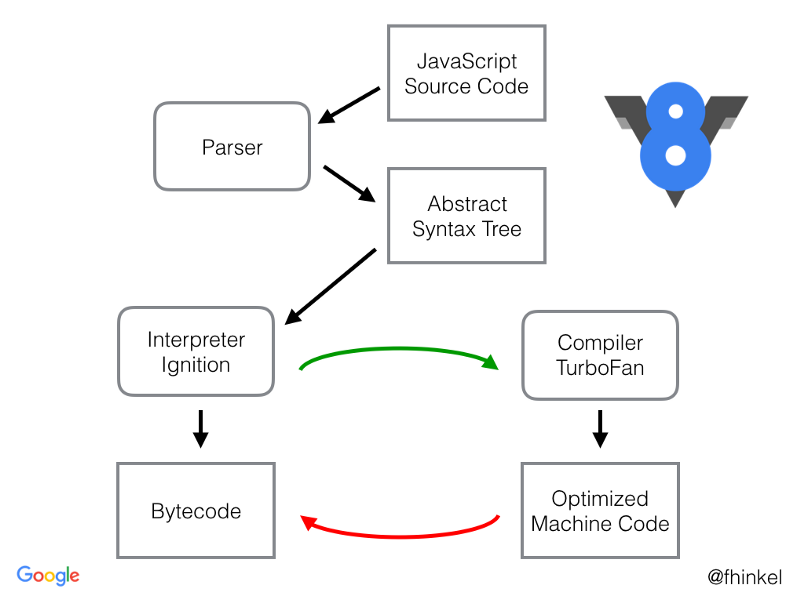
\includegraphics[width=\textwidth]{v8-architecture}
	\caption{V8 internal architecture}\label{fig:ast-v8-architecture}
\end{figure}

\subsection{User interace and state of the BC evaluator}\label{user-interface-and-state-of-the-bc-eval}

To keep the implementation consistent from the user perspective \textbf{BC} debugger should use the the same user-interface as the \textbf{AST}. There can also be visible distinguishing between the internal state of the language~(if the language is currently inside the \textbf{AST} or \textbf{BC} evaluation mode).

There is also need for the print current state of the \textbf{BC} stack machine which consists of the:

\begin{itemize}
	\item Current position inside code
	\item Stack content
\end{itemize}

Alongside the showing the current position there would be also need to show the function \textbf{BC} content. For this feature we can use the disassembler feature proposed in the first part of the analysis. Showing current position inside code can be implemented as an feature inside the \textbf{BC} disassembler but for the stack content there has to be implemented an separate tool~(function).

\subsection{Summary}

In order to improve bytecode debugging there is need for improving~(implementing the human-readable) disassembler. 

After analyzing the \textbf{GNU R} internal implementation of \textit{bcEval} function and the implementation of the \textbf{JS V8 VM} and Python VM there is definitely need to mark and put some condition for the marking of the bytecode instruction that the bytecode has been setted on that one. As long as there is focus on performance the bytecode debugger should in the best way put no overhead while it is not debugging. Looking into the internals of the V8 we can reuse the idea of making the separate instructions for bytecode debug flag which would call the neccesary debug routines~(as shown in the AST~debugger~\ref{AST-debugger}) and after that call the original instruction to keep functionality of BC~(needed to not break program integrity).

Finally there has to be done some showing of the internal status to end user. This consists of the printing the current position in the code and printing the stack content. For the current position in the code there can be reused the disassembler~(see~\ref{analysis-of-disassembler}) but for the dumping of the stack content there has to be implemented an separate tool.

\chapter{Realisation}

There are three different things which has to been done - disasembler, stack printer and finally the \textbf{BC} debugger. The BC debugger is using use the stack printer and disassembler so it make sense to implement the disassembler first.

\section{Implementation of the disassembler}\label{implementation-of-disassembler}

The whole project was structured that disassembler can be easily released~(to the \textbf{CRAN} repository) without the debugger. This is affecting the whole structuring of the project. The disassembler feature is made to be ready-to-deploy to the \textbf{GNU R} beta-testing codebase.

The main idea behind the disassembly rool was to write as much as possible code in the R language and just neccesary minimum in C for keeping the code simple. In the \textbf{GNU R} language there is the \textit{compiler} package written in R which contains the current \textbf{BC} compiler and \textbf{BC} disassembler~(very minimal - see~\ref{current-bc-disassembler}). As long as the contribution to the \textbf{GNU R} repository has very strict code styling rules which are much more relaxed for the 3rd party libraries inside \textbf{CRAN} repository decision was to make as much as possible inside the separate library which would be then published with some minimal changes to the main repository. Name of the package was decided to be the \textit{bctools}.

\subsection{User interface}

For more user friendliness of the \textbf{BC} print function there has been make an decision to use advantage of the \textbf{S3} class system~(see~\ref{R-Classes}). The old \textit{disassemble} function inside the \textit{compiler} package was kept almost intact. The only change that has been made there was putting class into the disasembly code. The name of the class has been decided to be the "disassembly". This allows us to have \textit{print.disassembly} function~(\textit{print} method of \textit{disassembly} class) inside our package which would be automatically dispatched once user call the \textit{print} function on the object if the \textit{bctools} package would be loaded inside user library.

The usage then changed from~(in the previous version / before the changes made in this thesis):

\begin{lstlisting}
#initialization
library(compiler)
f<-function(a) a+1
compiled <- cmpfun(f)

#disassembly
#  same output due internal to behavior of REPL as the
#    print(disassemble(compiled))
disassemble(compiled)

#generated output:
# list(.Code, list(8L, GETVAR.OP, 1L,
#   LDCONST.OP, 2L, ADD.OP, 0L,
#   RETURN.OP), list(a + 1, a, 1))
\end{lstlisting}


To the:

\begin{lstlisting}
#initialization
library(compiler)
library(bctools) #new package
f<-function(a) a+1
compiled <- cmpfun(f)

#disassembly
#  same output due internal to behavior of REPL as the
#    print(disassemble(compiled))
disassemble(compiled)


#generated output:
#
#  @ a
#  GETVAR              a
#  @ 1
#  LDCONST             1
#  @ a + 1
#  ADD
#  RETURN
#
\end{lstlisting}

\subsection{Instruction arguments}\label{instruction-arguments}
The \textbf{BC} instruction contains the integer code identifying it followed by variable number of arguments. These arguments can be of different types~(described in more detail bellow). 

The implementation of these operators is expecting arguments with different types~(definition is hardcoded inside compiler and evaluator function) but there is currently no list containing list of these 4 types for each instruction:

\begin{itemize}
	\item \textbf{CONSTANT} representing reference~(integer index) to the constant pool where is located constant expression~(can be either number or function)

	\item \textbf{BOOL} boolean value

	\item \textbf{INT} integer value

	\item \textbf{LABEL} label~-~jump target / reference~(integer index) to the code array itself

	\item \textbf{CONSTANT{\_}LABEL} variation~(extension) of the \textit{LABEL} which allow more than one referenced index
	
	represented as reference~(integer index) to the constant pool where is located an array containing the references~(integer indexes) to the code array itself
\end{itemize}

The \textbf{CONSTANT} parameter although can have two different meanings in the code. In the \textbf{GNU R} bytecode some of the arguments could be just whole expression~(e.g. a+b+c) kept due to usage in some corner cases during evaluation~( e.g. ADD instruction is in the most cases taking the two topmost arguments, just in these corner cases it is calling the other internal functions which are originally designed to work on the \textbf{AST} evaluator so they expect the expression as an input). Basically it means that these arguments are stored just because the internal implementation and contains the duplicate information. These two meaning should be distinguished inside the disassembler print so there has been put decision to split the \textbf{CONSTANT} parameter into the:

\begin{itemize}
	\item \textbf{CONSTANT{\_}DBG} - constant expression inside the argument used internally just for the corner cases~(technically containing duplicitous information)

	\item \textbf{CONSTANT} - regular constant expression used for most of common cases
\end{itemize}

So the final list of the argument types is:

\begin{itemize}
	\item \textbf{CONSTANT} representing reference~(integer index) to the constant pool where is located constant expression~(can be either number or function)

	\item \textbf{CONSTANT{\_}DBG} - constant expression inside the argument used internally just for the corner cases~(technically containing duplicitous information)

	\item \textbf{BOOL} boolean value

	\item \textbf{INT} integer value

	\item \textbf{LABEL} label~-~jump target / reference~(integer index) to the code array itself

	\item \textbf{CONSTANT{\_}LABEL} variation~(extension) of the \textit{LABEL} which allow more than one referenced index
	
	represented as reference~(integer index) to the constant pool where is located an array containing the references~(integer indexes) to the code array itself
\end{itemize}

\subsection{Annotation of instructions}
These 6 types should be printed in different way. There are 2 ways how to implement these behaviors in the bytecode disassembler. The first is to hardcode the behavior for the each instruction. This make sense for the compiler ( \textit{compiler} package ) and evaluator ( mostly \textit{bcEval()} function ) because they are basically generating or evaluating the instructions which does not need any anotation at all. On the other hand in our disassembly script only difference between printing these argument types would formatting of output. For this reason it makes a sense to write the code as much generic as possible. The best solution is to just take the definition and prints out the instruction according to its' definition.

In the compiler package there is already some annotation of the \textbf{BC} instructions in the form specifying the number of arguments for each instruction. After fully annotating all instruction by specifying each argument type, these values can be computed from the instruction annotation. This definition of the instruction parameters annotation also is more logically connected with the \textbf{BF} which generation and support functions are inside \textit{compiler} package than the disassembler~(would be just using this feature). Despite the fact that in the purpose of the work there has been idea that as much as possible code should be put inside the 3rd party library~(\textit{bctools}) it was decided to put the annotation inside the compiler package. This annotation of the instructions inside the \textit{compiler} package would also allow easier maintainance for the \textit{bctools} package because every time there would be added new instruction its definition has to be added in the \textit{compiler}. The argument annotation would now be part of the instruction annotation so even the disassembler would support then this instruction~(it would be reading the instruction definition from the \textit{compiler} package).

The \textit{compiler} package is made with the \textit{noweb} tool which is the tool to write documentation alongside with the code. Because of the fact that build command~(\textit{make}) is not written to re-generate the source code from \textit{noweb} each time the compiling is provided, each time this noweb source is changed there has to be run the \textit{make from-noweb} command inside the compiler package directory~(\textit{src/library/compiler}) to regenerate the C sources.

Example of the Instruction argument annotation inside \textit{compiler} package:
\begin{lstlisting}
<<opcode argument description>>=

SKIP.ARGTYPE<--1L
LABEL.ARGTYPE<-0L
CONSTANTS.ARGTYPE<-3L
CONSTANTS_DBG.ARGTYPE<-4L
BOOL.ARGTYPE<-5L
INT.ARGTYPE<-6L

Opcodes.argdescr <- list(

BCMISMATCH.OP = c(),
RETURN.OP = c(),
GOTO.OP = c(LABEL.ARGTYPE),
BRIFNOT.OP = c(CONSTANTS.ARGTYPE,LABEL.ARGTYPE),
POP.OP = c(),
DUP.OP = c(),
PRINTVALUE.OP = c(),
STARTLOOPCNTXT.OP = c(BOOL.ARGTYPE, LABEL.ARGTYPE),
    #  bool is_for_loop, pc for break
.... all remaining instructions ....
)
\end{lstlisting}

Calculating of the argument count array is done then by:

\begin{lstlisting}
Opcodes.argc <- lapply(Opcodes.argdescr, length)
\end{lstlisting}

\subsection{Instruction arguments and labels}\label{instruction-arguments-labels}

Label is form of representation of the reference to the code. It is used in the jumps through the code. Main \textbf{BC} array can store just one value itself so if there is an need for few jump locations~(e.g. like \textit{GOTO} operator) it is just value of the argument itself~(\textit{LABEL} type of argument). The switch operator could have also multiple locations where to jump so it is internally utilizing an \textit{CONSTANT{\_}LABEL} arguments type.

\subsection{Computing of labels}

To visualize the jumping locations in the diassembler there are usually showed labels in the code to specify target location~(usually incrementally numbered from the 1) and arguments are then in forms of references to these locations. These references are printed in the way that is has to be obvious that it is aiming to the specific location. This can be achieved using some specific symbol - e.g. {\$}1)~(reference to label with number 1). 
However there is no real direct information about these locations which should contain labels directly in the bytecode definition~(even the x86 code does not have these). Instead of it there are just references in the instructions to the code array, but we can compute the list of labels from these references. For generating this list there was done the two-pass linear lookup through code to generate auxiliary array containing the information direct information of number of the label~(the list is expressed as this array).

Steps to generate labels are then:
\begin{enumerate}
	\item Initialize auxiliary array with the size of code buffer. The each element has the default value representing, that there is no instruction which argument is pointing to that position.
	\item Go through all instruction in forward direction. For each argument if it contains any label~(see labels inside arguments~\ref{instruction-arguments-labels}) label then mark the according instruction on its location inside the auxiliary array.
	\item Go through the auxiliary array and set on each position marked as target for some instruction number of label. This number of label is calculated incrementally~(in the beginning set counter to 1, and on each marked position set the value of counter to the array and increment the counter)
\end{enumerate}

This array then would contain the information whether there is no label at the instruction or the label unique number.

Code used for computing labels:
\begin{lstlisting}
#first pass to mark instruction with labels
#labels is array that describes if each	Aq
#    instruction has label
n <- length(code)
#labels now contains -2=not used, -1=used
labels <- rep(-2, n)
i <- 2
instrCnt<-0 # count number of instructions
while( i <= n ) {
    v <- code[[i]]
    argdescr <- Opcodes.argdescr[[paste0(v)]]
    j <- 1
    while(j <= length(argdescr)){
        i<-i+1
        if(argdescr[[j]] == argtypes$LABEL){
            labels[[ code[[i]] + 1 ]] <- -1
        }else if(argdescr[[j]] == argtypes$CONSTANT_LABEL){
            v <- constants[[ code[[i]] + 1 ]]
            if(!is.null(v)){
                for(k in 1:length(v)){
                    labels[[v[[k]] + 1]] <- -1
                }
            }
        }
        j<-j+1
    }
    instrCnt<-instrCnt+1
    i<-i+1
}

#second pass to count labels
#loop through labels array and if
#   that instruction has label marked on it
#labels array now contains values:
#   -2=not used, -1=used, >0=index of label
i <- 2
lastlabelno <- 0;
while( i <= n ) {
    if(labels[[i]] == -1){
        lastlabelno <- lastlabelno+1
        labels[[i]] <- lastlabelno
    }
    i<-i+1
}
\end{lstlisting}

\subsection{Verbosity and formatting}

Bytecode compiled function has optionally the information about location of the source. These informations are not neccesary for the evaluation of the code but are good for human-readability~(see~\ref{Exprref-and-srcref}). Alongside with this there are also some of the instruction arguments which are used just for the reason of the internal implementation and have duplicate value~(see previous~chapter~\ref{instruction-arguments}). All of these information are not necessary to be displayed for the user for the basic information but it is nice for them to provide ability to display even these information. To provide this conditional ability to show more basic or more advanced information there has been put an decision to implement more levels of the verbosity in the disassembly tool.

The levels are:

\begin{itemize}
	\item \textbf{0} - display only source references~(if they are available, if they aren't print expression references instead)
	\item \textbf{1} - the same as 0 + display bytecode version and display expression references ( if they are available )
	\item \textbf{2} - the same as 1 + display every operand's argument~(including ones used just for debugging)
\end{itemize}

Default value can be pre-set by \emph{bcverbose} function~(provided in the \textit{bctools} package).

\subsection{Function types in the constant pool}

The constant expressions in the constant pool can of more 3 types:

\begin{itemize}
	\item regular~(ordinary) constant expressions~(e.g. numbers, array of numbers etc.)
	\item native functions~(calls to inside of the GNU R C implementation)
	\item BC compiler function code
\end{itemize}

There is no way how to print out the native functions because its structure is written and compiled inside the runtime core in C language and the R interpreter knows just it's location~(function pointer) to call. These functions are printed as an \textit{$<$INTERNAL{\_}FUNCTION$>$}. Alongside of these internal functions there are also stored the \textbf{BC} compiled functions which should be also printed out. The way how to do it is just say that this is the function and print out flag like \textit{$<$BYTECODE{\_}FUNCTION$>$}. The second approach is to be able to print it out nested with some indentation. The second described approach was chosen. To enable this feature there are 3 parameters in out disassembly tool:

\begin{itemize}
	\item \textbf{prefix} - the string prefix which is putted before each line printed in the whole function
	
	\item \textbf{depth} - current depthness of the recursion.
 	
	\item \textbf{maxdepth} - maximal depthness for recursion~(once it would reach this level, the \textit{$<$FUNCTION$>$} instead of calling the disassembly print would be shown in the output)
\end{itemize}

With these arguments it is possible to provide functionality disassembly recursiveness. Even though if the maxdepth would be set to the 0, the disassembly tool would print out just the \textit{$<$BYTECODE{\_}FUNCTION$>$} for every bytecode information~(the nested BC printing would be disabled).

\subsection{Printing functions}

One type of the constant expressions in the constant array are the functions written as an expression references~(non-byte-compiled and being able to potentially evaluate with \textit{eval} function inside \textit{src/main/eval.c}). These ones has to be printed in some user-friendly way which would not break the consistency of disassembly output. One way of printing the is to use the \textit{dput} function but they would be printed line by line which is not desired output. In order to make the arguments look as dense as possible~(and not break consistency and compactness of the disassemble function) there has been put decision to write the function in single line. There are 2 ways how to solve this:

\begin{itemize}
	\item Write an specific call into the \textit{print.c}~(\textit{src/main/print.c}) - \textit{deparse1} function
	\item Call an \textit{dput} to print out line-by-line into the buffer by \textit{capture.output} and after that make string modifications over this output.
\end{itemize}

The first approach is more clean in order of the code but as long as there has been put the decision to make just minimal amount of the changes into the C core of the language to be able to release the disassemble package the second way was chosen.

TODO: maybe add some good shit ( code example )

\subsection{Printing of different types}

In the application there are different types of the actions to print~(e.g. Constants, Operators etc.). The corresponding implementation of printing functions in the disassembler is named by the dump\textit{NAME}~(e.g. \textit{dumpConstant} ) convention. The complete list of types to print:

\begin{itemize}
	\item \textbf{Constant}
		
		used for printing any constant value
		
		description of the functionality of the whole operator is described in the following chapter subsection~(see~\ref{printing-constant-expressions})
		
	\item \textbf{Operator}
		
		used for printing the operator name
		
		The operator names are received by the \textit{bcinfo} function from \textit{compiler} package with the \textit{.OP}~(e.g.~\textit{ADD.OP}). The knowledge that it is operator is obvious so we do not want to print it. Because of it function for printing operands is extracting the \textit{.OP} suffix and printing just the actual name~(e.g.~\textit{ADD}).
		
	\item \textbf{Value}
	
		used for printing the \textit{INT} and \textit{BOOL} argument types
		
		printing the expression by calling directly the \textit{cat} function

	formatting notation - directly the \textit{NUMBER}~(e.g.~1)
		
	\item \textbf{Label}

	formatting notation - \$\textit{LABEL{\_}NO}~(e.g.~\$1)
	
	\item \textbf{SrcRef} a.k.a. \textbf{source reference}  
	
	formatting notation - \textit{SRCREF}~(e.g.~simple{\_}bc{\_}verbosity1.R{\#}4)
	 
	\item \textbf{ExprRef} a.k.a. \textbf{expression reference}
	
	formatting notation - $@$\textit{EXPRESSION}~(e.g.~$@a+1$)

	the expressions are stored in the constant pool so technically they are special type of the constant expressions. For printing them we can reuse then the print function for constant ones~(the \textit{dput} and eventually even \textit{print} functions has internal support for printing out the expression references). The only difference we need to print the $@$ as prefix. So final implementation of the print function is to dump $@$ to the output and then call the function for printing out the constant expression.
	
\end{itemize}

\subsection{Documenting of code}

Code itself was written to be self-explainable and easily readable with any developer for good maintainability. On top of that there was also written a lot of comments thorough the code.

From the user-perspectiwe there was created an user-documentation for R the package by the \textit{roxygen} tool~(the \textbf{GNU R} inbuilt documenting system). There are several ways for developer to rebuild the documentation:

There are three main ways to run \textit{roxygen}:
\begin{itemize}
 \item \textbf{roxygen2::roxygenise()}, or
 \item \textbf{devtools::document()}, if the \textbf{devtools} are used, or
 \item \textbf{rCtrl + Shift + D}, if the \textbf{RStudio} is used
\end{itemize}
 
The second listed~(calling \textbf{devtools::document()}) was used during an development of this package.

\section{Implementation of the bytecode stack printer}\label{implementation-of-stack-printer}

In order to implement the \textbf{BC} debugger we need to be able to print in user-friendly way the \textbf{BC} stack content~(see~\ref{user-interface-and-state-of-the-bc-eval}). The way how the implementation was designed was that it was written in the \textbf{C} language~(\textbf{GNU R} language core) a printing function capable of stack of current pointer.

\subsection{Stack definition}

Stack definition depends on the \textit{TYPED{\_}STACK} typedef conditional. If it is definied then the stack optimalization~(type of \textbf{unboxing}) is enabled so there can be stored even raw values on the stack alongside an boxing \textbf{SEXP} type. So then the types which could be stored on the stack are of type:

\begin{itemize}
	\item \textbf{int}
	\item \textbf{double}
	\item \textbf{RAWMEM} - additional piece of raw memory piece of length SEXP->ival~(in sizeof(SEXP))
	\item \textbf{SEXP} - internal representation of the boxed object storing any value
\end{itemize}
	
In case this \textit{TYPED{\_}STACK} is not defined it is just the boxed \textit{SEXP} value.

The definition of the stack element is here:

\begin{lstlisting}
#ifdef TYPED_STACK
typedef struct {
    int tag;
    union {
	int ival;
	double dval;
	SEXP sxpval;
    } u;
} R_bcstack_t;

... other definitions ...
#else
typedef SEXP R_bcstack_t;

... other definitions ...
#endif
\end{lstlisting}

Luckily there is implemented an macro \textit{GETSTACK{\_}PTR} which would return us an boxed \textit{SEXP} type equivalent no matter if the value in stack is boxed or unboxed. This would allow us to write the stack print function much easier without any need of separate handling of unboxed values.

\subsection{Printing of the stack values}\label{printing-stack-values}

This functionality is completely written in \textit{C} and it was designed to reuse as much code as possible. 

In analyzing printing of the stack values there has been realized that it is not possible to use the \textit{print}~(\textit{PrintValue} call in \textbf{C}) function because it is dumping output in the very spread out manner~(array and object items are printed each at separate line). The better output formatting has the \textit{dput} function, but it is written inside \textit{base} package~(written in \textbf{R} instead of \textbf{C}). After the research what is \textit{dput} doing under hood it was observed that is calling the internal \textbf{C} implementation of the \textit{do{\_}dput}~(inside \textit{src/main/deparse.c}) which unfortunately cannot be reused without any changes. The reason is that it is internally caling the \textit{deparse1} function with the parameter to internally evaluate the promises. However this printing should not evaluate any promises because they could  potentially change the output of the bytecode~(they can have side effects). To disable this feature~(promise evaluation) we can call the \textit{deparse1} function with first argument setted to \textit{SHOWATTRIBUTES} | \textit{DELAYPROMISES}. The function would instead of evaluating them just print the $<$promise$>$ text signalizing that there is promise in that particular element.

\subsection{RAWMEM stack type tag}

Items on the stack are formatted in C-style array but in case the \textit{TYPED{\_}STACK} is defined the one of the types can be \textit{RAWMEM}. In that case the following memory contains the some raw data so we cannot call to these items regular function for printing elements and instead of we have to skip~(jump over) that chunk of memory.

The data on the stack would be in our function printed with the first line pointing to the top of the  stack. Because of this this reason we want to print the stack from the top to the bottom. The \textit{RAWMEM} type however is pointing to the followed data instructions and not the previous. This means that if we would be printing the stack from the end~(top) we would not be able to decide whether the next position contains raw memory or regular stack value.

To be able to detect this we created the auxiliary \textit{LOGICAL}~(internal representation of binary inside \textbf{GNU R}) array which would contain boolean flag if the value is printable. Tis means we also needed to add one linear pass through the stack to fill in this array. This pass is in the forward order~(from bottom to top of the stack) so we are able to tell whether the memory is the raw or not. 

This caused that whole algorithm to dump the stack needs to have two passes:

\begin{itemize}
	\item \textbf{First pass} from bottom to top to fill out the auxiliary array
	
			sets the TRUE value on the visited value. If the visited value is the RAWMEM type, then mark the n following~(size parameter of the RAWMEM cell) cells FALSE

	\item \textbf{Second pass} from top to bottom to actually print out the values on the stack
	
			works in the way that skip values for every place where the are auxiliary value is set to FALSE. If TRUE then look to the tag~(if \textit{TYPED{\_}STACK} available) if is \textit{RAWMEM}, then print $<$rawmem of size \%d$>$ otherwise call the print function for the value~(see~\ref{printing-stack-values}).
\end{itemize}

If there is \textit{TYPED{\_}STACK} not defined it means that the there is no support for \textit{RAWMEM} which would induce that all of the values are printable. In that case the auxiliary array is useless but we still decided to keep this auxiliary array to be able to use as much same code for every case as possible. This would induce one linear lookup of the array which is not neccesary but in term of performance it is just constant slowdown. This function would be used mainly in debugging we are not concerned about the performance that much~(the \textbf{VM} would be sitting and waiting for user input at some point of the time anyways).

For style formatting we chose to print just simply $<$rawmem of size \%d$>$ text to specify that there is raw memory chunk on the stack.

\subsection{Persisting stack pointers}\label{printing-stack-values}

In regards of the \textbf{BC} stack information there are currently these~(global) variables representing the current state.
 
\begin{itemize}
\item \textbf{R{\_}BCNodeStackBase} representing the bottom of the stack
	\item \textbf{R{\_}BCNodeStackTop} pointing to the current top of the stack
	\item \textbf{R{\_}BCNodeStackEnd} representing the end of allocate space for the stack~( stack is represented internally as an array)
\end{itemize}

Which satisfies equation 

$R{\_}BCNodeStackBase < R{\_}BCNodeStackTop < R{\_}BCNodeStackEnd$

To be able to print values on the current evaluating bytecode stack we need to know when function stack frame starts and ends~(\textit{R{\_}BCNodeStackBase} points to the beginning of the whole stack and not to the beginning of current evaluated function). For knowing this information we don't have enough information in these variables so we decided \textbf{R{\_}BCNodeStackFnBase} which would point to the beginning~(bottom) of the current evaluated function so after that we would have an memory range in within is the current evaluated stack frame. As long as this variable is internally represented as C global variable but it is used in function context~(mimicking of the CPU function local stack frame behavior) we need to add this variable also to the handling the context~(in the \textit{src/main/context.c}).

\section{Conditional breakpoints}\label{conditional-breakpoints}

Due to lack of the the ability of the conditional breakpoins which are simple and user-friendly there has been put decision to add simple user-friendly \textit{breakpoint()} function which fires the debugger functionality on the spot. It is inspired by the \textbf{JS} \textit{debugger;} command, but instead of being an separate command which would be big change in the language parser we decided it to be just an callable function.

This function is simply modifying the \textit{RDEBUG} feature of the current evaluating environment and resetting the temporary bytecode variables (\textit{R{\_}BrowserLastCommand} and \textit{browserfinish} member of function context). This command works like every other function, so it is called with new environment. On the other side we want to change variables of not this environment but the evaluated function, so there has to be done the environment lookup for the parent function context.

\begin{lstlisting}
SEXP attribute_hidden do_breakpoint
	(SEXP call, SEXP op, SEXP args, SEXP rho)
{
    Rboolean oldrdebug;
    oldrdebug = RDEBUG(rho);
    SET_RDEBUG(rho, 1);
    R_GlobalContext->browserfinish = 0;
    R_BrowserLastCommand = 'n';

	...other support for bytecode 
		debugger ( described below )...

    return R_NilValue;
}
\end{lstlisting}

Usage example:
\begin{lstlisting}
#setting up the bytecode
options(keep.source=TRUE)
debugVerbose(TRUE)
enableBCDebug(TRUE)
library(compiler)

#evaluated function
f<-function(){
  for(x in 1:5){
    if(x == 3){
	  breakpoint();
	}
  }
}
compiled <- cmpfun(f)
compiled()
\end{lstlisting}


\section{Implementation of the debugger}

The main purpose of this work is enable to do the bytecode debugging. In order to do debugging we need to visualize the current bytecode internal state of the evaluating function~(debugger work in the each function separately) which consists of:

\begin{itemize}
	\item Position inside bytecode
	\item Bytecode stack content
\end{itemize}

The position inside bytecode can be printed alongside with the bytecode content~(we can use already implemented bytecode disassembler~\ref{implementation-of-disassembler}). For the second part we already implemented the stack printer function.

\subsection{Main idea}

The main idea behind the debugger implementation is to maintain the same functionality and user interface as the current \textit{AST} implementation.

\subsection{Global design}

The idea used behind the debugger implementation is inspired by the \textbf{JS V8 VM}~(see~\ref{bcdebug-implementation-in-v8}). It is to replace the original instruction with special breakpoint instruction together with backuping~(saving) the original instruction alongside the bytecode. This would enable the dispatching of bytecode debug features with evaluating the same code while not causing any performance overhead in case the code is not debugged.

This feature is still experimental so it is by default disabled. Managing this state is done in \textit{src/main/debug.c} by \textit{R{\_}is{\_}bc{\_}debug{\_}enabled} and \textit{do{\_}enableBCDebug}~(exposed into R as \textit{enableBCDebug}).

Example~(notice the \textit{enableBCDebug} call):
\begin{lstlisting}
options(keep.source=TRUE)
library(compiler)
enableBCDebug(TRUE)

f<-function(a){
    c<-a+1
    d<-c+a
    c-d
}
compiled <- cmpfun(f)
debug(compiled)
compiled(2)
\end{lstlisting}


\subsection{Instruction for debugging}\label{instruction-for-debugging}

To be able to dispatch breakpoints there has been created an specialized set of debug instructions. For dispatching breakpoint on the instruction the original instruction is replaced with it's equivalent~(according to the number of arguments, see below) breakpoint one. The debugging instructions are:

\begin{itemize}
	\item \textbf{BREAKPOINT0}
	\item \textbf{BREAKPOINT1}
	\item \textbf{BREAKPOINT2}
	\item \textbf{BREAKPOINT3}
	\item \textbf{BREAKPOINT4}
\end{itemize}

There has been put the decision to make an instruction for each number of the arguments instead of one generic instruction. All the functions which are working with the debug instructions are then setting the debug on the specific instruction and code for checking the breakpoint~(\textit{bcInstrIsBreakpoint} function in the \textit{compiler} package) which would be affected by this decision of creating more separate instruction. On the other hand there are already other parts of the R code~(translating bytecode instructions to function pointers and vice versa through \textit{bcEncode}/\textit{bcDecode}, bytecode disassembler etc.) which works with the instruction argument counts inside the current C code. These ones would remain intact and working with any change. This decision would also allow better forward compatibility because this is allowing less code duplication~(in the case adding instruction with more than 4 arguments it would mean changing just that two places. Even though if these changes would not be applied in future which should never happen~(but we eventually can think even this case) the interpreter \textbf{BC} functionality would be intact and would not crash. The only affected feature would be non-working disassembler and debugger~(setting the next breakpoint) features. It is very bad and critical but not the worst case scenario of the whole interpreter crashing.

The other possible option~(which was not chosen) would have been to have just one debug instruction for whole bytecode set of instructions. This solution would save some possible BC instruction space~(for now at least 4 instructions) and allow more simple implementation of the setting/unsetting breakpoint~(no need to look up original instruction argument count) but would add more complexity to the all functions working with the \textbf{BC} instructions argument count~(\textit{bcEncode}/\textit{bcDecode}/disassembler etc.).

\subsection{Storing of the original instruction when the breakpoint is setted}\label{storing-original-instructions}

There is need to somehow remember the original instruction in case the breakpoint is set on the instruction~(the original instruction is overwritten by the corresponding breakpoint one but we still need to execute the original one alongside with the debugger features). The function can have more than one instruction replaced with the debug so there cannot be stored just one original instruction for each function but there has to be option ton store one for each position in the BC code array.

The idea behind implemented solution is on the first change~(first setting of the breakpoint) make an deep copy of the whole \textbf{BC} code array and attach it into the linked list of the bytecode~(see internal representation of the bytecode~ref{R-internal-bc-representation}). Once this is done we can set or unset the breakpoint on any instruction without worrying of losing any information. The representation of the garbage collector is treating the bytecode as a generic linked list~(it's code is inside src/main/memory.c) so the there are any changes needed for keeping the memory consistent.

\subsection{Setting and unsetting debug instruction}\label{setting-and-unsetting-debug-instruction}

To be able to set~(and unset) the debug instruction on the bytecode there has been created an \textit{bcSetBreakpoint} function inside compiler package~(but can be very easily moved into another one if neccesary because it is just dependent on the C core function and the instruction annotation which is already exported through \textit{bcinfo} function). It has support for both setting and unsetting the instruction~(parameter \textit{is}). This function is internally used in the \textbf{BC} debugger which internally needs the informations where has been placed the new breakpoint instruction. For this case it returns the array containing the positions of newly set instructions. 

Function implementation:
\begin{lstlisting}
bcSetBreakpoint <- function(code, pos, is=TRUE) {
  if (typeof(code)=="closure")
    bc <- .Internal(bodyCode(code))
  else
    bc <- code
  if (typeof(bc)!="bytecode") 
    stop("Internal error - code is not bytecode")

  bc <- .Internal(disassemble(bc))
  bcode <- bc[[2]]
  newbcode <- rep(bcode) #replicate original bytecode

  #loop through bytecode over instructions and find 
  #   matching instruction
  setpos <- 2
  repeat{
    if(!(setpos < length(bcode) && setpos <= pos)) break
    setpos <- setpos + 1 + Opcodes.argc[[bcode[setpos]+1]]
  }

  .Internal(modifybcbreakpoint(code, setpos-1, is));

  setpos-1
}
\end{lstlisting}

The function is exposed to the end user so it needs to be fail-proof. The \textbf{BC} code array does not contain just the instruction operands but also its arguments which cannot be rewritten in any case scenario. The only way how to check whether the value is operand or its instruction  is going from the beginning of the code array instruction by instruction. The function would then find the first avaThe way how the function was designed was then it would set or unset~(depending on the parameter \textit{is})

 it would firstly find the first instruction which position~(index) >= parameter \textit{pos}. This feature would prevent user from the corrupting of bytecode array~(marking the position of the argument instead of operand). The nice side-effect is that it would allow us to to elegantly solve \textbf{next step} feature of debugger. The debugger could have had just take the position of the current evaluating instruction and just add the 1 no matter how many arguments has the current instruction because it would all the time set the following instruction.

As we can see in the code the function is calling internally the \textit{modifybcbreakpoint}. It taking the bytecode function representation~(first argument), position~(second argument) and flag if the breakpoint should be set or removed~(third argument). The function is at first check if there is backup of the original bytecode~(to save the potential old representation of the code~(see storing of original instructions~\ref{storing-original-instructions}). If not, it would create an shallow copy of the bytecode representation assigned to the function call~(so basically just this specific function call would have an modified breakpoint code). The bytecode array copy would then be appended to this shallow function definition copy. This way would keep the memory overhead the minimal~(shallow copy is small and the only bytecode array is once duplicated and assigned to it's copy). After this is done there could have been provided the setting / unsetting the breakpoint on the array. Setting is done by looking to the definition of the instruction to it's number of arguments and unsetting is done just by copying the value from the second bytecode array~(with saved instructions) which contains every time unmodified instructions. As you can notice there is no removing of the auxiliary array in case the last debug instruction was removed. This decision was made because the memory overhead of keeping the auxiliary array is minimal and the removing would add additional complexity to this function.

\subsection{Listing breakpoints}\label{listing-breakpoints}

In order to manage the breakpoint status there has been implemented a \textit{bcListBreakpoints} function for listing the setted ones.

\begin{lstlisting}
options(keep.source=TRUE)
library(compiler)
library(bctools)

f<-function(a){
    c<-a+1
    d<-c+ac
    c-d
}

compiled <- cmpfun(f)

#set breakpoints

 #this breakpoint would be set into position 12,
 # because at 11 is argument and 
 # the implemented functionality is setting 
 # the breakpoint in that cases 
 # to the first following instruction
bcSetBreakpoint(compiled, 11);
 #14 is regular instruction
bcSetBreakpoint(compiled, 14);

#print the current function 
# - notice the (BR) in the instruction
print(disassemble(compiled),verbose=2)

#print the bytecode instructions 
# - see the 12 and 14
print(bcListBreakpoints(compiled))
\end{lstlisting}

\subsection{Setting the next breakpoint}\label{setting-next-breakpoint}

Consequential instruction does not necessary mean the following instruction right next in the bytecode array due to labels. The breakpoint for the next instruction can be either one of these:

\begin{itemize}
	\item following in the bytecode array
	\item at the position which were instruction labels pointing at~(see types of labels~\ref{instruction-arguments-labels})
\end{itemize}

To support this feature there has been developed the\textit{bcSetNextBreakpoint} function inside the \textit{compiler} package. There has been also written internal bindings wrapper inside the \textbf{C} package~(call to the \textbf{R} code) in the function \textit{Rf{\_}breakOnNextBCInst}. 

The code is checking all possible locations for the jump locations also with the check if there is already one breakpoint~(in that case it is not adding). If there is no breakpoint on the location it is then putting there breakpoint. For placing the breakpoint it is using the internal call to the C function \textit{modifybcbreakpoint}~(see~\ref{setting-and-unsetting-debug-instruction}).

It is also internally generating an array of added breakpoint locations which is then returning. This feature is then used in the internal implementation of the breakpoint instruction in the C core~(this returned array is used to keep tracking of the added breakpoints).

The function code:

\begin{lstlisting}
#simulate next behavior with breakpoints
# returns the vector of added breakpoints
bcSetNextBreakpoint <- function(code, pos){
    if (typeof(code)=="closure")
        bc <- .Internal(bodyCode(code))
    else
        bc <- code
    if (typeof(bc)!="bytecode")
        stop("Internal error - code is not bytecode")

    bc        <- .Internal(disassemble(bc))
    bcode     <- bc[[2]]
    origbcode <- bc[[3]]
    consts    <- bc[[4]]


    tryAddBreakpoint<-function(pos, ret){
        #if there is no breakpoint at position pos, 
        # set breakpoint to that position and add 
        # append this position into list ret
        # finally return the list ret 
        #  of breakpoint positions
        if(!(pos %in% ret) && pos <= length(bcode)){
            opcode <- bcode[pos]
            if(!bcInstrIsBreakpoint(opcode)){
                .Internal(modifybcbreakpoint(code, 
                			pos-1, 
                			TRUE));
                ret <- append(ret, as.integer(pos-1))
            }
        }
        ret
    }

    #handle adding breakpoint to the first instruction
    #  we need this after entering 
    #  bcEval in case of RDEBUG == 1
    ret <- vector(mode="integer", length=0);
    if( pos < 1 ) {
        return(tryAddBreakpoint(2, ret))
    }

    opcode    <- origbcode[pos]
    descr     <- Opcodes.argdescr[[opcode+1]]

    #iterate over all parameters of instruction
    i <- 1
    while( i <= length(descr) ){
        if(descr[[i]] == LABEL.ARGTYPE){
            #if it is label, add breakpoint to target
            # instruction and append its position to 
            # return array
            ret <- tryAddBreakpoint(
            			origbcode[i + pos] + 1, 
            			ret)
        }else if(descr[[i]] == CONSTANTS_LABEL.ARGTYPE){
            #the label arguments are through 
            # constants array
            labelvals <- consts[[ origbcode[i + pos] + 1 ]]
            if(!is.null(labelvals)){
                for( v in 1:length(labelvals) ){
                    ret <- tryAddBreakpoint(
                    		labelvals[[v]]+1, 
                    		ret)
                }
            }
        }
        i <- i+1
    }
    #if instruction has no labels, add breakpoint to 
    # its following instruction
    if(opcode != RETURN.OP && 
    	opcode != RETURNJMP.OP && 
    	opcode != GOTO.OP) {
        ret <- tryAddBreakpoint(
        	pos + 1 + length(descr), ret)
    }

    ret
}
\end{lstlisting}

\textit{bcInstrIsBreakpoint} function is used for checking if the instruction code is breakpoint. Internally it is just wrapper over the condition to limit the code duplication~(this check is used on more places in the whole code).

\begin{lstlisting}
bcInstrIsBreakpoint <- function(x) {
  x == BREAKPOINT0.OP ||
    x == BREAKPOINT1.OP ||
    x == BREAKPOINT2.OP ||
    x == BREAKPOINT3.OP ||
    x == BREAKPOINT4.OP
}
\end{lstlisting}

\subsection{Support in the disassembly tool}\label{debugger-support-in-disassembly}

To visualize the set breakpoints there has been added an support into the disassembly tool. The R disassembly script was modified to getting an an 3 arrays as an bytecode input~(added an field with backup of all bytecode array). So the arrays now contain the constant array, code array possibly containing breakpoints and original code array which never contains any breakpoint instruction. The original array is returned every time no matter if the code array is modified or not~(in case not modified there is returned the same array twice). 

This means that we can just simply modify the disassembler to go always through the original array. Then for every instruction we would be checking in the code array~(which possibly contains breakpoints) if there is breakpoint or not. In case there is we would just simply print an mark \textit{(BR)} as prefix for the instruction name to signalize that this instruction contains breakpoint.

Loading an arrays with breakpoints:
\begin{lstlisting}
#can contain BREAKPOINT[0-9] instructions
code_breakpoint   <- x[[2]]
#never contains BREAKPOINT[0-9] instruction
code              <- x[[3]]
#constant buffer
constants         <- x[[4]]
\end{lstlisting}


Checking for breakpoint:
\begin{lstlisting}
if(grepl("^BREAKPOINT[0-9]+\\.OP$", code_breakpoint[[i]])){
    instrname <- paste0("(BR) ", instrname)
}
\end{lstlisting}

\subsection{Temporary and regular breakpoints}

Currently there are two types of the breakpoint inside the bytecode:

\begin{itemize}
	\item temporary breakpoint
	\item regular breakpoint
\end{itemize}
	
The regular ones are used for user-defined breakpoint~(by calling \textit{bcSetBreakpoint} function from {compiler} package). Once bytecode interpreter reaches them it breaks and show the interface for debugger.

The temporary ones are used on the other hand for handling debugger commands. They are implemented with the same instruction except they are also held their locations on the bytecode local stack~(variable in which points global \textit{R{\_}BCtmpBreakpoints} also kept through context in \textit{src/main/context.c}). This value contains an array in which each elements is pointing to the location of the breakpoint. These breakpoints always point to the instruction succeeding current the evaluated one~(see~\ref{setting-next-breakpoint}.

In order to keep the garbage collector satisfied and because it is not possible to store the in the local protection stack~(\textit{PROTECT}/\textit{UNPROTECT} function), there has been decided to dedicate the one field on the bytecode stack for this array. The \textit{R{\_}BCtmpBreakpoints} is then pointer~(\textit{SEXP*} type) to this location which allows changing of this variable while modifying the bytecode body. Changing this array and not keeping an new one also reflects the fact that the changes inside the bytecode code array are also made in-place in destructive manner.

\subsection{Implementation of the breakpoint instructions}\label{implementation-of-breakpoint-instruction}

The reason why there are implemented separate breakpoint instructions for each number of instruction arguments is just because they would have different annotation which would contain the number of arguments. Basically the breakpoint instruction contains the information of the number of its arguments in order to not break the structure of bytecode. The code itself inside all of them would be the same. This means that it can be simply generalized by writing an macro for all breakpoint instruction and calling this macro for each instruction.

The code for instructions ended up like:

\begin{lstlisting}
    OP(BREAKPOINT0, 0): DO_BREAKPOINT();
    OP(BREAKPOINT1, 1): DO_BREAKPOINT();
    OP(BREAKPOINT2, 2): DO_BREAKPOINT();
    OP(BREAKPOINT3, 3): DO_BREAKPOINT();
    OP(BREAKPOINT4, 4): DO_BREAKPOINT();
\end{lstlisting}

The breakpoint instructions algorithm~(\textit{DO{\_}BREAKPOINT} macro) is:

\begin{itemize}
	\item Remove all temporary breakpoints from the bytecode
	\item Call debug browser
	\item Set the debug flags~(RDEBUG or mark next bytecode instruction for debgging)
	\item Call the original instruction
\end{itemize}

As you can see in the time of calling the browser there are all temporary breakpoints removed from the bytecode. It means that just the regular user-defined breakpoints would the printed to the output~(see~\ref{debugger-support-in-disassembly}) which is desired behavior because we do not want to print the user breakpoints which are used just for implementation of debugger.

\subsection{Handling of the recursive character of the bytecode}

As you can see the debugger implementation while going through the code is modifying the breakpoint code with adding an temporary breakpoins to support breaking on the next instruction~(see~\ref{setting-next-breakpoint}). In the time of the evaluating instruction there can be set temporary breakpoints somewhere in the code and if this instruction is CALL to the current instruction we have to delete them. In that case the algorithm is to 

TODO this shit is fucked up, it is erasing also regular breakpoints

\subsection{Threaded and non-threaded design of the application}

Because of the speedup there is implemented support for the THREADED code which would remove the main loop from the bytecode instruction evaluation loop~(see~\ref{Computed-GOTO}). So basically there has to been two different systems which had to be analyzed and modified to support the jumping to the different direction~(jump for calling the original instruction inside the \textit{DO{\_}BREAKPOINT} macro).

\paragraph{THREADED{\_}CODE defined}

In this case the changes were minimal. It required just adding an macro \textbf{BREAKPOINT{\_}GOTO{\_}ORIGIN{\_}OP} for an switching to the instruction defined in the backup array~(\textit{inst} argument). Because of the implementation design of the bytecode instruction in case of the instruction operand it is holding internally position of it's label to jump to~(see~\ref{Computed-GOTO}). All it is doing is then jumping into the location defined in passed instruction value.

\begin{lstlisting}
#define NEXT() (__extension__ ({ \
	currentpc = pc; goto *(*pc++).v; \
	}))

#define BEGIN_MACHINE  NEXT(); 
	init: { loop: switch(which++)


#define BREAKPOINT_GOTO_ORIGIN_OP(inst) do{ \
     __extension__ ({goto *(*(inst)).v;}); \
  } while(0)
\end{lstlisting}


\paragraph{THREADED{\_}CODE not defined}

On the other hand in case of not defined support for \textit{THREADED{\_}CODE} situation is more complicated. In that case the whole evaluator design is one big loop. The loop originally had big switch~(beginning defined in \textit{BEGIN{\_}MACHINE} macro) which was deciding which instruction according to the value of operand~(*op). We changed this behavior that we loaded operand into variable, placed another jump label~(\textit{jmp{\_}opcode}) and after that decided which instruction has to be evaluated according to the value of that variable. In the case of executing BREAKPOINT and evaluating original instruction~(through \textbf{BREAKPOINT{\_}GOTO{\_}ORIGIN{\_}OP}~\ref{}) we set the auxiliary variable~(\textit{jmp{\_}opcode}) to the desired instruction code and jumped into jump label which we added~(\textit{jmp{\_}opcode}) which would dispatch the another instruction code~(without increasing program count pointer etc.).

\begin{lstlisting}
#define NEXT() goto loop

#define BEGIN_MACHINE  loop: \
	currentpc = pc; \
	jmp_opcode = *pc++; \
	do_instruction: switch(jmp_opcode)

#define BREAKPOINT_GOTO_ORIGIN_OP(inst) do{ \
    jmp_opcode = *(inst); \
    goto do_instruction; \
  } while(0)
\end{lstlisting}

\subsection{Handling of the debugger user input}

The original environment browser has inbuilt support for handling and modifying the debugging~(step into, next step, continue etc.) via the user input~(defined in \textit{src/main/main.c}) implemented by setting up the \textit{RDEBUG} flag altogether with \textit{R{\_}BrowserLastCommand} variable on the evaluated environment. The intend of implementing bytecode debugger interface was to reuse as much of this feature so the bytecode debugger is managed also through these variables. Bytecode interpreter provides the more status information, so the user interface has been extended by these commands:

\begin{itemize}
	\item \textbf{bc} - print current bytecode with the position~(internally calling \textit{R{\_}printCurrentBCbody})
	\item \textbf{bcstack} - print current bytecode stack~(internally calling \textit{R{\_}printCurrentBCstack})
\end{itemize}

Implementation in \textbf{ParseBrowser}:
\begin{lstlisting}
    ...
	other commands
	...
	}else if (!strcmp(expr, "bcstack")){
        rval = 2;
        RCNTXT* cntxt = GetBCDebugContext();
        if(R_BCIntActive)
            R_printCurrentBCstack(
            		R_BCNodeStackFnBase, 
            		R_BCNodeStackTop);
        else
            Rprintf("Debugged context is not bytecode\n");
    } else if (!strcmp(expr, "bc")) {
        rval = 2;
        RCNTXT* cntxt = GetBCDebugContext();
        if(R_BCIntActive)
            R_printCurrentBCbody(R_BCbody, R_BCpc, FALSE, 1);
        else
            Rprintf("Debugged context is not bytecode\n");
    } else if () {
    ...
	other commands
	...
    }
\end{lstlisting}


%Both of these functions are called by the global bytecode arguments (\textit{R{\_}BCbody}, \textit{R{\_}BCpc} etc.) which can be changed~(conditional breakpoints supported through \textit{trace} function are evaluated through R code which can cause another bcEval call which change these variables). 

%\begin{lstlisting}
%int olddisablebc = R_disable_bytecode; \
%R_disable_bytecode = TRUE; \
%do_browser(body, CALL_FRAME_FUN(), R_NilValue, rho); \
%R_disable_bytecode = olddisablebc; \
%\end{lstlisting}

\subsection{Default behavior of the bytecode debugger}

The whole bytecode debugger engine was designed in it's default way for the user to behave in the most similar way as the current AST one. The only difference is printing \textit{"debugBC"} instead of printing \textit{debug} in the beginning of the each line used for user command input~(environment browser). Making the debugger output behaving as much similar as the current AST implementation is beneficial for other dependent software which is relying on the specific output format~(such as IDEs etc.).

\subsection{Verbose mode of bytecode debugger}

The bytecode debugger on the other hand can jump in much more granular way~(not according to the changes of expression references but step for each bytecode instruction) and also have additional state information~(bytecode stack). Support for this feature was implemented in this thesis through function \textit{bcVerbose()} called with parameter TRUE or FALSE.

Once the verbose mode is enabled the debugger is stepping through each bytecode instruction. For printing current state there is reused the calling \textit{R{\_}printCurrentBCbody} in \textit{src/main/eval.c} internally dispatching \textit{print} method of bytecode object from the \textit{bctools} package (called with \textit{select} parameter to show current instruction and \textit{peephole} turned to show just surrounding area across the current instruction). 

This flag is internally represented through the boolean \textit{R{\_}DebugVerbose} global variable.

To support this feature there has been implemented function \textit{printBCStatus()} for printing the bytecode interpreter status.

Its code is:
\begin{lstlisting}
void printBCStatus(){
    Rprintf("     --- Evaluating bytecode --- \n");
    R_printCurrentBCbody(R_BCbody, R_BCpc, TRUE, 1);
    Rprintf("     -------- Stack dump ------- \n");
    R_printCurrentBCstack(R_BCNodeStackFnBase, R_BCNodeStackTop);
}
\end{lstlisting}

As you can see the code is reusing the \textbf{bytecode disassembler}~\ref{implementation-of-disassembler} and \textbf{stack printer}~\ref{implementation-of-stack-printer}.

\subsection{Initial entry points to the bcEval functions}

Because the in the bytecode implementation there are no checks for the RDEBUG flag due to performance~(avoiding condition instruciton every each evaluated bytecode instruction) there is need for setting the bytecode instruction~\ref{setting-next-breakpoint} in order to dispatch bytecode functionality manually.

Currently there are two cases in which this scenario has to be handled.

\begin{itemize}
	\item At the beginning - the bytecode function was just called
	\item At the return from the function call
\end{itemize}

The first case is handled in the start of the bytecode evaluation \textit{bcEval} function. In this case we just call the \textit{Rf{\_}breakOnNextBCInst} which call internally  \textit{bcSetNextBreakpoint} function from the \textit{compiler} package. In the start point of the function evaluation \textit{R{\_}execClosure}~(R function implementation is wrapped in closure) is condition if the function has \textit{RDEBUG} flag enabled and there are met criteria to start debugging, the \textit{RDEBUG} flag is set in the current evaluated environment. In the \textit{AST} evaluator there is then checked the environment \textit{RDEBUG} flag. The user interface \textit{debug}, \textit{debugOnce} etc. are changing the function flag~(not the environment one) which implies that there cannot be changed the \textit{RDEBUG}  by calling debug on the function while executing the function~(this implies any instruction so also the any function all from this code). It means that for support the current behavior the only place where is need to add BREAKPOINT instruction is in the beginning of the \textit{bcEval}.

Code in the beginning of the \textit{bcEval} function:
\begin{lstlisting}
if(RDEBUG(rho)){
  ptrdiff_t diff = pc - codebase;
  Rf_breakOnNextBCInst();
  codebase = BCCODE(body);
  constants = BCCONSTS(body);
  pc = codebase + diff;
}
\end{lstlisting}

The other entry point would be used just in case of the implementation of the conditional breakpoints~\ref{conditional-breakpoints}. In this case there has to be done the two changes for fully support this feature.

\begin{itemize}
	\item If the breakpoint modified the state of the evaluated bytecode function~(the function was not in debug mode and now is due to calling breakpoint), add the debugging instruction to the next following instruction~(see~\ref{conditional-breakpoints}).
	\item The function described above can possibly change the internal structure of bytecode object structure so there has to be done the update of the changed internal variables after call to the function
\end{itemize}


Marking following instruction as breakpoint:
\begin{lstlisting}
SEXP attribute_hidden do_breakpoint
	(SEXP call, SEXP op, SEXP args, SEXP rho)
{
	... setting debugging flags ( described above ) ...

    if(!R_is_bc_debug_enabled() && R_BCIntActive)
  warning(_("Calling breakpoint in the BC 
  		while bytecode debugger disabled"));

    /* Support for bytecode debugger */
    if(R_BCIntActive && !oldrdebug){
      R_RemoveBCtmpBreakpoints(
          R_BCbody, *R_BCtmpBreakpoints);
      Rf_breakOnNextBCInst(
          R_BCbody, R_BCpc, R_BCtmpBreakpoints);
    }

    return R_NilValue;
}
\end{lstlisting}

The \textbf{CHECK{\_}ADD{\_}BREAKPOINT} function is used for resetting the internal variables~(after the) state in the bcEval function. This reset it done in case of the \textit{DEBUG} flag on the function is enabled~(the \textit{do{\_}breakpoint} is turning this flag on). This added function is adding some overhead in case of debugging but in this case we are not worried about the performance. The bigger concern is adding one variable check even if the function is not in \textit{DEBUG} mode.
\begin{lstlisting}
#define CHECK_ADD_BREAKPOINT(pcdiff) do { \
    if(RDEBUG(rho)){ \
      ptrdiff_t diff = *((BCODE**)R_BCpc) - codebase - 1; \
      *((BCODE**)R_BCpc) = BCCODE(R_BCbody) + diff + 1; \
      codebase = BCCODE(R_BCbody); \
      constants = BCCONSTS(R_BCbody); \
      pc = *((BCODE**)R_BCpc) + pcdiff + 1; \
   } \
} while(0)
\end{lstlisting}

\chapter{Testing and future work}

The each 3 implemented parts of this thesis were tested separately. The best case scenario was to make set of automated tests which would test out the all of the implemented features.

\section{Bytecode disassembler}

The main part of the work was done as the separate \textbf{GNU R} package~(named \textit{bctools}). The R package system has it's testing system which runs every file in the \textit{tests} directory and checks its the return code. 

The main test parts include:
\begin{itemize}
	\item \textbf{basics.R} - basic functionality (printing the different cases - for loop, switch command, while loop etc.)
	\item \textbf{advanced.R} - advanced functionality
	\item \textbf{closure.R} - printing function closure
	\item \textbf{switch.R} - switch command
	\item \textbf{peephole.R} - peephole parameter
	\item \textbf{bcverbose.R} - verbose parameter
	\item \textbf{bcversion.R} - check if the current GNU R BC version is the supported one in this package~(see~\ref{R-internal-bc-representation})
\end{itemize}

Because of the simplicity the tests were written without any testing framework. Nowadays if the test fails there is not any more detailed information where the error occurs inside the file. To support this functionality it is possible modify the tests to use \textbf{test{\_}that} framework which supports naming the tests and printing the name in case of it's fail. 

\section{Bytecode debugger}

The \textbf{BC} debugger tests was done to make sure that there are no bugs in the code. The testing was done manually altogether with the writing of the some automated tests. Automated testing was done by step by step simulation of the step-into~(\textbf{"s" command} in the browser) by modifying beginning of the \textbf{Rf{\_}ReplIteration} function~(found in \textbf{src/main/main.c}). 

The modified function:
\begin{lstlisting}
int Rf_ReplIteration(
	SEXP rho, 
	int savestack, 
	int browselevel, 
	R_ReplState *state
  )
{

  ... variables initialization ...

  if(!*state->bufp) {
    R_Busy(0);
    if(browselevel){	
    	/* environment browser is on */
      strcpy((char*)state->buf, "s\n");
    }else{
      if (R_ReadConsole(
      	  R_PromptString(browselevel, state->prompt_type),
            state->buf, 
            CONSOLE_BUFFER_SIZE, 
            1)
             == 0)
        return(-1);
    }
    state->bufp = state->buf;
  }

  ... end of the function ...

}
\end{lstlisting}

Altogether with these changes there was made an script~(modification of the test feature from the \textit{R CMD test} command) to utilize the R package test files as testing examples. The tool was comparing the output with and without an bytecode debugger support enabled and trying to simulate the same output as normal. Although this tool was not 100\% successful because internally the tests~(tested on the test directory from the \textit{bctools} package) was using catching output with it's internal feature. Running the debugger in this function meant that there was infinite recursion~(catching output which causes another catching of the output). This testing can be considered just partially successful, because it was not able to run across any of the input test cases. 

Next to this automated testing this feature was tested manually, which results were considered successful.

\subsection{Effectiveness of testing}

During the tests there has been observed numerous issues. Some of them were caused by the oversight during analyzes of the \textbf{BC} compiler and/or evaluator. Example of these are:
\begin{itemize}
	\item handling of the \textbf{SWITCH} command arguments - lack of support for the \textbf{CONSTANT{\_}LABEL} type - this feature support has to be also done into the disassembler code
	\item memory issues caused by \textbf{Garbage collector} due to forgotten support for the added global variables (such as \textbf{R{\_}BCNodeStackFnBase})
	\item memory issue caused by modification of the body variable while duplication of the current evaluated one~(see~\ref{setting-and-unsetting-debug-instruction}) - solved by pushing this variable onto the BC stack
\end{itemize}

\subsection{Side effects of the scripts}

There are limited options to debug the memory errors inside the language \textbf{VM}~(and generally any \textbf{C} code) and finding these errors are even more difficult when the  R code is evaluated - in that case the code is internally represented as \textit{SEXP} type parameter in the \textit{eval} or eventually as an bytecode in the \textit{bcEval}. 

To be able to better understand whether some of the memory issues which occurred were caused by the injected R code and not other changes there has been made decision to rewrite some of the parts to not use \textbf{R} call to the \textbf{compiler} package but use just native \textbf{C} implementation. These parts are not having the full functionality as their \textbf{GNU R} counterparts and were not fully tested. Although of this they can be useful for future performance improvements so they are included in the attached DVD.

These parts of code are:
\begin{itemize}
 \item \textbf{Rf{\_}breakOnNextBCInst}
 \item \textbf{do{\_}BCdisasm} used in \textbf{R{\_}printCurrentBCbody} function
\end{itemize}

\section{Conditional breakpoints}

Technically conditional breakpoints are in term of the code part of the debugger support so even the testing was done altogether other testing of the bytecode debugger support.

\section{Future work}

\subsection{Push into working repository}

The big part of the planned future part of the future work is to collaborate with the \textit{GNU R} core team to pushing this work into it's development and potentially even the production code. After this would be done and considering the number of people using \textbf{GNU R} language~(the estimation in the 2013 was approx 2 millions), the work done in this thesis would have big worldwide effect to lot of the people.

\subsection{Merging the bctools package into the compilers}

The \textbf{bctools} package was developed independently as an separate disassemble feature with the minimal changes to the \textbf{GNU R} VM core. This tool was also used in the debugger which is part of the \textbf{VM} core. When the debugger would be deployed it is suggested to merge the \textbf{bctools} package into the \textbf{compiler} while the source of the bctools one is relatively short~(approx. 600 lines). The reason why this was not already done but just proposed here as future work is that it would allow to deploy the disassembler into the working branch faster and eventually give a user-feedback for improvements before merging inside the \textbf{compiler} package and deploying the debugger.

\subsection{GNU R Memory optimization}

Some of the parts of the errors which were done and fixed during the development of this thesis were memory-based. During investigation of these errors there has been noticed one thing. The core of the \textbf{GNU R} language is heavy dependent on the linked list memory data structure. During the modern computer implementation of the memory system this can cause a lot of memory cache misses which affect the performance. The most straightforward way to do this is to use an smallvector technique~(inspired by an \textbf{llvm} compiler) but the more appropriate way would be to do analysis of whole \textbf{GNU R} memory subsystem optimization with focus on cache locality.

\setsecnumdepth{part}
\begin{conclusion}

The GNU-R language is one of the most popular scientific language using worldwide with not just scientific community but also non-scientiscs. For better evaluation performance it's VM is internally supporting the bytecode alongside with old-fashioned and slow AST interpreter. Since nowadays options for debugging the bytecode were very limited. The disassembler shows just the plain array of instructions and constant buffer and the debugger is internally dispatching the AST debugger so it is not going through the same code as while not debugging. 

In this thesis there has been proposed and implemented changes which contains the user friendly easy human readable bytecode disassembler. The second part is about the implementation of the native debugger support for bytecode evaluator. As the additional fun feature there has been added support for conditional breakpoints in the code in very user-friendly manner inspired by the JavaScript breakpoint command.

In the beginning there is brief introduction to the problem and the motivation part. Following is the analysis of the current implementation of the \textbf{GNU R} bytecode disassembler and debugger alongside with the comparison to similar tools and features in other languages \textbf{VM}. After that there are described implementation details of the work. Firstly there is described implementation of the disassembler followed by the stack printer. As an addition it is described the implementation of the conditional breakpoint support. Finally there is debugger where is shown reuse of two previously described features. The end of the work contains chapter about the testing of all features altogether with possible future work and improvements.

All the features were developed and tested and are included on the enclosed DVD. Personally it was a very good experience to work on the real language \textbf{VM} while implementing feature which would use millions of people. The work done in this thesis can be considered as successful.

\end{conclusion}


\bibliographystyle{iso690.bst}
\bibliography{mybibliographyfile}

%\setsecnumdepth{all}
\appendix

\chapter{Acronyms}
% \printglossaries
\begin{description}
	\item[VM] Virtual Machine
	\item[BC] Bytecode
	\item[GC] Garbage collector
	\item[AST] Abstract syntax tree
	\item[IR] Intermediate representation
	\item[OO] Object oriented
	\item[OOP] Object oriented programming
	\item[JIT] Just in time
	\item[REPL] Read-Eval-Print-Loop
	\item[UI] User interface
	\item[ARM] Advanced RISC Machine, originally Acorn RISC Machine
	\item[CRAN] The Comprehensive R Archive Network
	\item[GCC] GNU Compiler Collection
	\item[TDD] Test driven development
\end{description}


\chapter{Contents of enclosed DVD}

%change appropriately

\begin{figure}
	\dirtree{%
		.1 readme.txt\DTcomment{instruction for the file}.
		.1 analysis\DTcomment{analysis of other implementations}.
		.1 examples\DTcomment{implementation examples directory}.
		.2 cond{\_}breakpoint\DTcomment{conditional breakpoint examples directory}.
		.2 r{\_}breakpoints\DTcomment{bytecode debugger examples directory}.
		.2 r{\_}disassembly\DTcomment{bytecode disassembler examples directory}.
		.1 noncomplete{\_}functions\DTcomment{analysis of other implementations}.
		.1 bctools\DTcomment{the bctools package directory}.
		.1 r{\_}src\DTcomment{modified GNU R source}.
		.1 thesis\DTcomment{the thesis source code directory}.
		.2 DP{\_}Saska{\_}Ales{\_}2018.pdf\DTcomment{the thesis text in PDF format}.
		.2 DP{\_}Saska{\_}Ales{\_}.tex\DTcomment{the thesis text in \LaTeX{} format}.
	}
\end{figure}

\end{document}
